\section{Introduction}


[++ Simulate the junction behaviour... ++]

[++ mcphase calculates both the IV curve and tha phase path (?) of the junction (outside the scope of the present paper) but only for a single value of alpha_rf ++]

A Josephson junction is a quantum mechanical device composed of two superconducting electrodes separated by a weak link \cite{Barone:1982}.
For currents lower than a critical value $I_C$, the device behaves as an uninterrupted superconductor and coupled electrons (Cooper pairs) can cross the weak link without any voltage drop.
[ALT+++ Coupled electrons (Cooper pairs) can cross the weak link without any voltage drop, at least until the current reaches a critical value $I_C$ (dc Josephson effect)..+++]
When the current is further increased, single electrons originated by the breaking up of Cooper pairs begin to traverse the weak link. The potential difference $V$ between the two superconducting films becomes $\neq 0$ and a state is reached where the junction behaves as a resistance.

Besides its current practical applications, the Josephson junction is important from a physical point of view because it has been the first device showing quantum mechanical effects on a macroscopic scale.

In modern Josephson junctions the weak link usually has the form of a thin insulating tunnel barrier (SIS junction) \cite{Gurvitch:1983}, a normal metal film (SNS junction) \cite{Benz:1995} or a physical nanoconstriction (ScS junction) \cite{Cybart:2015, DeLeo:2016}. Josephson junctions have found wide usage in several research fields, for example as building blocks for RSFQ digital electronics  or quantum computers \cite{Likharev:1991}, or as very sensitive magnetometers (SQUIDs) and radiation detectors \cite{Maggi:2006b, Granata:2015}.

But the most successful application of Josephson junctions is surely in voltage metrology.
A microwave radiation of frequency $f$ can phase lock the junction current, producing the so-called Shapiro-steps, i.e., current steps at the quantized voltages $V_n$, 

\begin{equation}
	V_n = n \frac{h}{2 e} f, \quad n = 1, 2, ...
\label{eq:voltage_steps}
\end{equation}

where $h$ and $e$ are the Plank constant and electron charge, respectively. This ac Josephson effect is at the basis of the quantum voltage standard that since 1987 replaced the previous voltage standard based on Weston cells.

%% However, only in the second half of the 80’s, the development of the reliable Nb/Al-AlO,/Nb fabrication process made it possible to reach quantized voltages of $1$ and $10$~V, suitable for direct dc voltage calibration. These devices were based on large series arrays of thousands of SIS Josephson junctions (here SIS stands for superconductor-insulator-superconductor, where Nb is the superconducting film and the Al0, layer is the insulating tunneling barrier of the junction).

%% The Josephson voltage standard at the $1$ and $10$~V levels that were the state-of-the-art implementation at the time and were deployed only in very few labs wordwide, required a very careful engineering of the microwave distribution lines within the many arms in which the Josephson arrays were divided. 

An important research topic at the beginning of the '90s was related to finding ways to increase the amplitude of the current steps induced by the microwave radiation. In fact, the stability of the lock between the junction phase and the applied microwave bias, and therefore its insensitivity to noise events which might switch the junction from one quantized level to another, which is a crucial problem for voltage standard applications, is strongly dependent on the step amplitude \cite{Kautz:1987}.

To increase the step amplitude, a non-sinusoidal microwave signal may be used.
In 1990 Monaco showed that, in the limit of a voltage-biased junction, when two phased microwaves of frequencies $f$ and $2 f$ are added together, the rf-induced current steps have normalized amplitudes larger than those predicted for a standard sinusoidal radiation \cite{Monaco:1990}. 
Experiments on the so-called ``biharmonic drive'' readily confirmed, at least in part, these conclusions, probably because the samples could not be properly considered as voltage biased \cite{Andreone:1991, Andreone:1992}.

Extending further the idea, Monaco showed that the rf-induced current steps of a voltage-biased junction could become as large as the junction critical current for a microwave radiation composed of a train of periodic delta functions.
However, in practice a voltage bias configuration does not properly model a real junction, which usually should be considered as current biased.
Further, a delta function wave shape is only theoretical and cannot be reproduced in experiments. This led to the idea to investigate what happened to a current-biased Josephson junction irradiated by a more realistic pulsed microwave signal \cite{Maggi:1996, Maggi:1997}. And this investigation is the object of the present work.


\section{Computational context}
\label{computational-context}

A first attempt to solve this problem was made by using an electronic analog simulator \cite {Henry:1981}, that could compute the $I-V$ characteristic of a current-biased junction in the framework of the Stewart-McCumber RSJ junction model \cite{McCumber:1968, Stewart:1974}.
The analog simulator was very fast and simple to use, and pairing it to a \href{http://www.hpmuseum.net/display_item.php?hw=7}{Hewlett Packard 7475A pen plotter} it could produce in just a few seconds beautiful plots of the $I-V$ characteristics of the junction as a function of the simulated microwave signal.\footnote{Unfortunately, after 25 years and two relocations, I could not manage to find pictures of the simulator nor the original HP 7475A plots.} The real problem with this approach was that, even if the electronic simulation was very fast, it took ages to measure by hand from the paper plots the amplitude of the rf-induced steps visible on each $I-V$ curve.

A different approach was necessary and I decided to write a FORTRAN program to solve numerically the nonlinear second-order differential equation that models the junction behaviour \cite{McCumber:1968, Stewart:1974}. The idea was to calculate the $I-V$ curves of the junction as a function of the pulse amplitude $\alpha_\mathrm{rf}$ for a given set of junction parameters $\beta$, $\Omega$ and $\rho$. To ease comparison of the results for different sets of parameters, normalized units have been used throughout the calculations \cite{McCumber:1968, Stewart:1974}. Usually, around $100$ different $I-V$ characteristics for increasing values of $\alpha_\mathrm{rf}$ were calculated for a for a given set of junction parameters.

The first versions of the FORTRAN program were compiled under DOS 6.22 with \href{https://winworldpc.com/product/microsoft-fortran/5x}{Microsoft Fortran 5.1} and run on what was then a state-of-the-art PC, probably a Compaq Deskpro 486 with a math coprocessor, that was shared among several users of the lab. 
However, after a few attempts the limitations of a standard PC for such a task soon become evident. A new simulation started automatically on late evenings and took the entire night to be completed. Unfortunately, people still using the PC late in the evening, often inadvertently stopped the background process (it was DOS and Windows 3.11 after all, multitasking was still barely usable) or simply shut the machine down without checking if there was some other running job. At the end, I was able to to complete a single simulation run only every two or three days! 

Luckily, after a few weeks of these mostly unsuccessful attempts, a colleague [that was also the sysadmin of his research group,] proposed me to use four Digital workstations running Digital UNIX, or more probably ULTRIX, for my own simulations. The machines were heavily used by his research group during working hours but sat mostly idle overnight. If I could manage to finish my runs before the start of the new work day, I was free to use this idle time for my simulations. My colleague gave me a quick crash course on UNIX and I was ready to go.\footnote{I should still have my notes somewhere.} Porting my FORTRAN program from DOS/Microsoft Fortran 5.1 to UNIX Fortran was a snap, and I also quickly managed to learn how to use FTP to transfer the configuration files needed by the simulations and the output files containing the results of the simulation back and forth from the DEC machines to my desktop machine (at that time, I was one of the \emph{happy few} to have a personal computer sitting on my own desk).

The real problem now was how to analyse all this data. A manual analysis like that needed by the electronic simulator was impractical, so I decided to try the recently released Microsoft Visual Basic 1.0 to write a program that took the nightly output files and calculated automatically the size of the rf-induced steps visible on the calculated $I-V$ characteristics as a function amplitude of the rf drive, $\alpha_\mathrm{rf}$.
Everything worked flawlessly.

So at the beginning of each day I had 4 different sets of files coming from the four DEC machines, three of them were made by keeping $\beta$ and $\Omega$ constant and changing the value of $\rho$, i.e., the (normalized) width of the pulse signal [++ CHIARIRE CHE OGNI NOTTE VENIVANO CAMBIATI I VALORI DI BETA E OMEGA ++]. The fourth simulation was made with exactly the same parameters but using a standard sinusoidal drive and was used to compare the results obtained with a standard sinusoidal microwave signal with those obtained with progressively shorter pulses.
I FTPed these files from the DEC workstation to my desktop computer and I run the Visual Basic program on each data set to quickly get a summary file containing the size of the quantized current steps for reference sinusoidal drive and for the three simulated junctions subjected to progressively shorter current pulses. The results of months of calculations were summarized in a paper published on the Journal of Applied Physics \cite{Maggi:1996}.


\section{Digging into code}

Finding the original sources of this project was easy and complex at the same time. I am the type of person that likes organisation, and I try keep all my past projects on my main work computer. So finding the original sources was only a question of finding the right directory where the project was stored.
Problems arise when I started to look at the different files. There were several directories, with many files with widely different names and dates, trying to find and order in that chaos seemed at first impossible. Normally I would have found many notebooks full of detailed handwritten notes for that project. Unfortunately, a couple of years ago most of my work notebooks were damaged by a water leak in my basement, and could not be recovered. So the only option was to look at the files one by one. Luckily modern operating system have many often little known tools that can greatly ease the work with files, macOS in particular offers QuickLook which allows to quickly browse through tens and hundreds of files at the touch of the spacebar.

%%some with  misleading names such as \textsf{old} or \textsf{obsolete}, which one was older? (turns out that \textsf{obsolete} is \emph{older} that \textsf{old}).

After a thorough inspection of the directories of the project I leaned that: (1) my first attempts with the numerical simulations used the more accurate McDonald-Johnson model \cite{McDonald:1976}, and that I switched to the simplified Stewart-McCumber RSJ junction model \cite{McCumber:1968, Stewart:1974} because it allowed much faster and efficient calculations; (2) file names reflected what the programs actually did, and in the same directory I could have a file ending with a "t" that provided a textual output and the same files ending with a "g" that gave a graphical output. Having many files differing only for a couple of \textsf{DEFINES}s might seem crazy today, when graphical interfaces and ultra-fast and ultra-confortable text editors with access to regular expressions allow to change a file in just a few seconds, but probably at that time it was the fastest, albeit inefficient, way of working with source code; (3) all source files had an header containing detailed notes about the type of program, the compiler, the type of output, and what probably mattered more, the dates of first and last revision of the source file (Fig.~\ref{fig:source-header}), and that eased much the analysis of the different versions of the FORTRAN source files; (4) the initial versions of the FORTRAN programs were monolithic, there was only one source file containing the whole code (around 1.000 lines of FORTRAN), only at a later moment good computing practice led me to divide the monolithic code into several source files that were compiled and linked together using a \textsf{Makefile} (but I will not delve into it here).

%===============================================================================
\begin{figure}[tb]
	\centering
	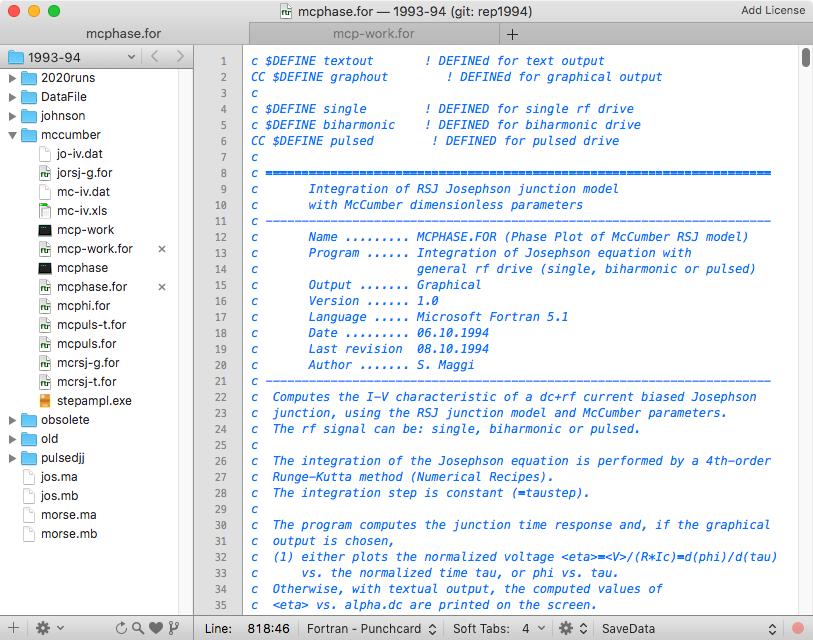
\includegraphics[width=0.75\textwidth]{source-header.png}
	\caption{Header of one of the FORTRAN source files.}
	\label{fig:source-header}
\end{figure}
%===============================================================================


A great tool that I used heavily was \href{http://meldmerge.org/}{Meld}, an open source tool for all current operating systems that can perform a two- and even a three-way comparison of files and directories. At the beginning it might seem confusing and hard to use, but when one gets the handle of it it becomes and invaluable tool to analyse computer code. Using \href{http://meldmerge.org/}{Meld} I quickly realized that the two main source files were \textsf{mcphase.for} and \textsf{mcp-work.for} (Fig.~\ref{fig:meld-comparison}), both located in the \textsf{mccumber} directory.

%===============================================================================
\begin{figure}[bt]
	\centering
	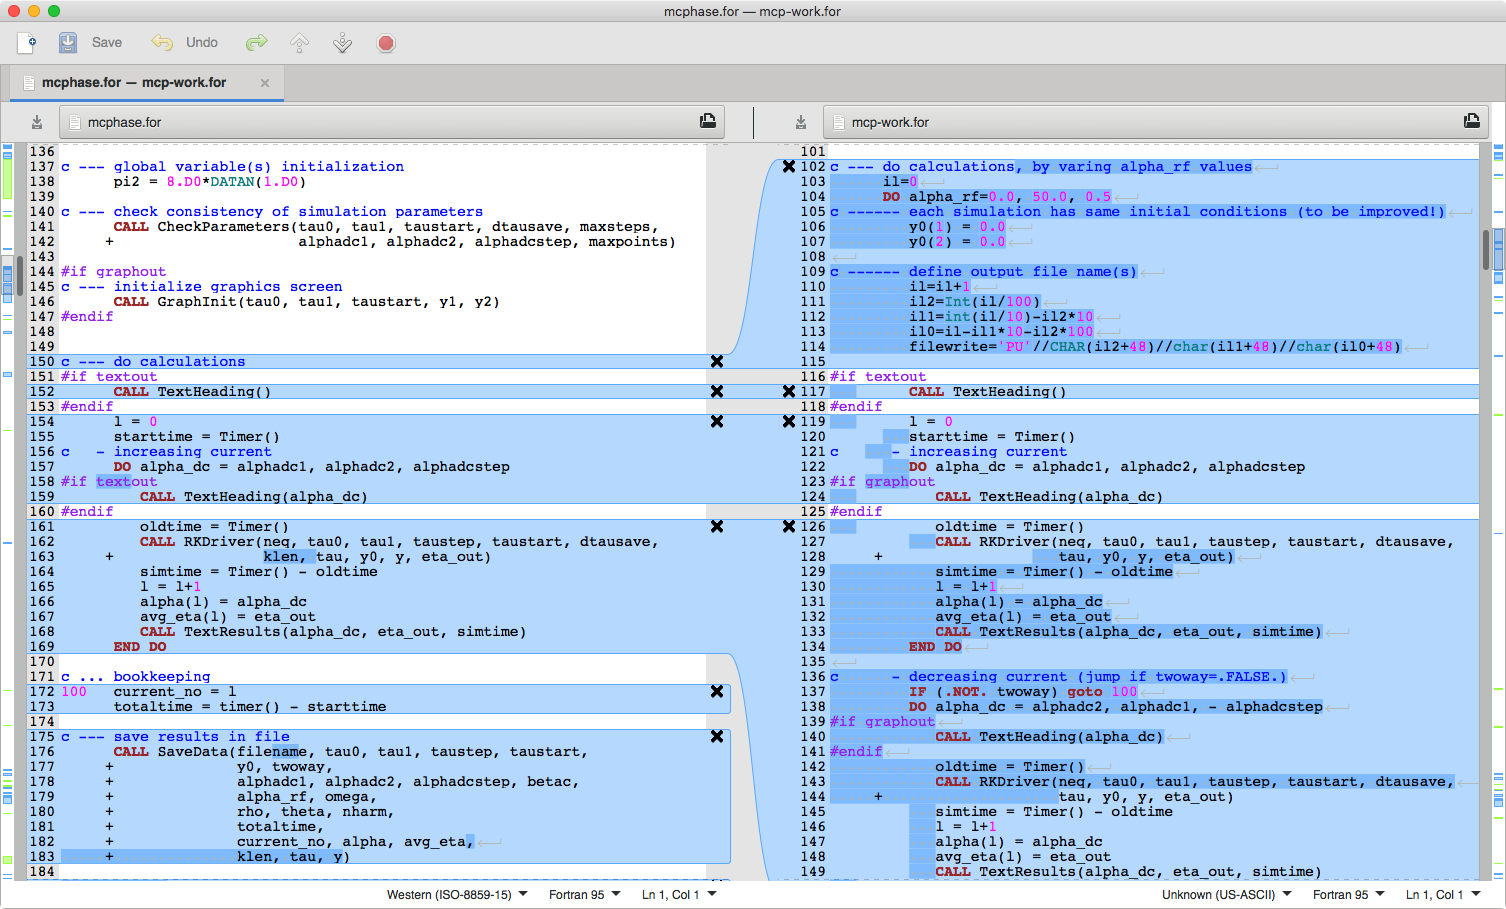
\includegraphics[width=0.75\textwidth]{meld-comparison.png}
	\caption{Meld...}
	\label{fig:meld-comparison}
\end{figure}
%===============================================================================


The former performed a simulation for a single value of $\alpha_\mathrm{rf}$, so it used a DOS batch file to perform simulations for several values of $\alpha_\mathrm{rf}$, renaming the output file containing the results of each simulation, \textsf{iv.out}, using a consistent naming scheme.
%for each value of $\alpha_\mathrm{rf}$, copied a \textsf{.dat} input file containing the proper set of simulation parameters into a file with a standard name, \textsf{iv.dat}, run the simulation and at the end renamed the output file containing the results of the simulation, \textsf{iv.out} so that it has the same basename of the original \textsf{.dat} input file.
This approach was typical of DOS and was also very inefficient and error prone, since each day it required to write a long series of \textsf{.dat} input files that differed only by the value of $\alpha_\mathrm{rf}$, updating correspondingly the long DOS batch file that controlled the night calculation (Fig.~\ref{fig:batch-file}.

%===============================================================================
\begin{figure}[tbh]
	\centering
	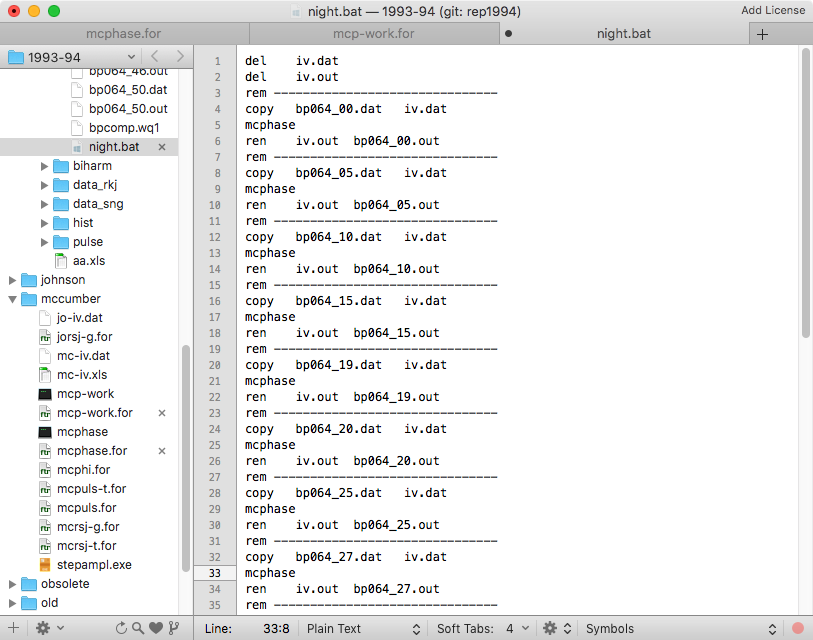
\includegraphics[width=0.75\textwidth]{batch-file.png}
	\caption{Batch file...}
	\label{fig:batch-file}
\end{figure}
%===============================================================================


On the other hand, \textsf{mcp-work.for} automatically cycled across a predefined set of values of $\alpha_\mathrm{rf}$, producing a different output file for each value of $\alpha_\mathrm{rf}$. It was clear that this was the source code ported to the DEC workstations. 
Unfortunately, I could not find the source file used o these machine, probably I ported my DOS/Microsoft FORTRAN 5.1 to Digital UNIX working directly on the workstations, and I never thought to copy back these sources since they could not work on my PCs.
Luckily, FORTRAN is very stable an it was very easy to port again both \textsf{mcphase.for} and \textsf{mcp-work.for} so that it worked on a modern machine.

As for the Microsoft Visual Basic 1.0 code, there were only two versions of the Visual Basic analysis programs and the differences between them seem minimal, so I decided to stick with the initial version.


\section{Porting Microsoft FORTRAN to UNIX}

Porting \textsf{mcphase.for} and \textsf{mcp-work.for} to the XXI century so that they could be compiled with a modern \textsf{gfortran} compiler was very easy, thanks to the stability of the language across different versions and platforms. Essentialy only a few tweaks to the source code were needed.


\subsection{Preprocessor directives}

For reasons that go beyond my understanding Microsoft Fortran 5.1 did not use standard \textsf{cpp} or \textsf{fpp} preprocessors directives (the latter is the de facto standard Fortran preprocessor) \cite{Boyanski:1992}, but used a a slightly different syntax (Fig.~\ref{fig:preprocessor}). Luckily, all was needed was to comment out all the \textsf{\$DEFINE} lines in the header section and to replace throughout the code Microsoft Fortran 5.1 \textsf{DEFINE} blocks with standard \textsf{cpp} blocks (Fig.~\ref{fig:preprocessor}). 


%===============================================================================
\lstset{
    language = C,
    basicstyle = \tiny\bfseries\ttfamily,
    tabsize = 4,
    frame = lines,
    framesep = 1em,
    framexleftmargin = 1em,
    backgroundcolor = \color{ultralightgray},
    keywordstyle = \color{darkred}\bfseries,
    morekeywords = {$DEFINE, $if, $endif, defined},
    deletekeywords = {for}
}
%===============================================================================
\begin{figure}[b]
\centering

\begin{minipage}{0.48\textwidth}
\textbf{(a)}
\begin{lstlisting}
$DEFINE textout			! DEFINEd for text output
c $DEFINE graphout		! DEFINEd for graphical output

c $DEFINE single        ! DEFINED for single rf drive
c $DEFINE biharmonic    ! DEFINED for biharmonic drive
$DEFINE pulsed			! DEFINED for pulsed drive

$if defined (graphout)
	...
$endif
...
...
$if defined (textout)
	...
$endif
...
$if defined (pulsed)
	...
$endif
\end{lstlisting}
\end{minipage}
%
\hfill
%
\begin{minipage}{0.48\textwidth}
\textbf{(b)}
\begin{lstlisting}
CC $DEFINE textout		! DEFINEd for text output
c $DEFINE graphout		! DEFINEd for graphical output

c $DEFINE single        ! DEFINED for single rf drive
c $DEFINE biharmonic    ! DEFINED for biharmonic drive
CC $DEFINE pulsed		! DEFINED for pulsed drive

#if graphout
	...
#endif
...
...
#if textout
	...
#endif
...
#if pulsed
	...
#endif
\end{lstlisting}
\end{minipage}

\caption{Preprocessor directives in (a) Microsoft Fortran 5.1, (b) modern \textsf{cpp} preprocessor.}
\label{fig:preprocessor}
\end{figure}
%===============================================================================


Now the right directives are chosen at compile-time, by running for example the following command,

%===============================================================================
\lstset{
    language = bash,
    basicstyle = \small\bfseries\ttfamily,
    tabsize = 4,
    frame = none,
    framesep = 2em,
    framexleftmargin = 1em,
    backgroundcolor = \color{ultralightgray},
    keywordstyle = \color{darkred}\bfseries,
    deletekeywords = {for}
}
%===============================================================================
\begin{lstlisting}
$ gfortran -cpp -Dtextout -Dsingle -o mcp-work mcp-work.for
\end{lstlisting}
%===============================================================================

to run the \textsf{cpp} preprocessor before compilation of \textsf{mcp-work.for} with \textsf{gfortran}, selecting code that produced textual output (\textsf{-Dtextout}) and performed calculations with the the single (sinusoidal) rf drive (\textsf{-Dsingle}).



\subsection{Filenames}

Fortran 77 did not support dynamic memory allocation and required programmers to use fixed-length arrays and strings. Strings were used rather sparingly in FORTRAN, so that was not a big deal. The exception in my my code was for the name of the files containing the simulation parameters and the results of the calculations, which was defined as a 50-byte long string.

%===============================================================================
\lstset{
    language = Fortran,
    tabsize = 6,
    frame = none,
    framesep = 2em,
    framexleftmargin = 1em,
    backgroundcolor = \color{ultralightgray},
}
%===============================================================================
\begin{lstlisting}
	CHARACTER*50   filename
\end{lstlisting}
%===============================================================================


Under DOS that was not a real problem, since DOS truncates file names to 8 characters (plus three characters for the extension) and excess characters were ignored, but under UNIX file names have no real limitations,\footnote{255 characters for the name of the file and 4096 characters for the path} and having these 50 characters long filenames, mostly composed by spaces, was ugly and, what matters most, complicated file management, in particular when using a command line interface.
The solution is simple, FORTRAN now has the \textsf{TRIM} function that removes all trailing blank characters from a string, so whenever a file is opened for reading or writing, it is sufficient to apply \textsf{TRIM()} to the \textsf{filename} variable, as shown here

%===============================================================================
\begin{lstlisting}
	OPEN (UNIT = 10, FILE = TRIM(filename)//'.dat', STATUS = 'OLD')
\end{lstlisting}
%===============================================================================


\subsection{Edit descriptors}

Microsoft Fortran 5.1 used the backslash \textbackslash{} edit descriptor to prevent the addition of a line break at the end of a \textsf{WRITE} instruction.\footnote{http://userweb.eng.gla.ac.uk/peter.smart/com/981124.htm}
Modern Fortran compilers do not support this peculiar edit descriptor, and return an error,  \textsf{unexpected element '\' in format string}. To avoid this error, it is sufficient to remove the backslash edit descriptor from all \textsf{WRITE} instructions that include it.


\subsection{Date and time}

Microsoft Fortran 5.1 has two separate intrinsic subroutines to return the current date and time.
In particular,

%===============================================================================
\begin{lstlisting}
	CALL GETDAT(iyr, imon, iday)
\end{lstlisting}
%===============================================================================

saved the date in the two-byte integer variables textsf{iyr}, textsf{imon} and textsf{iday}, while 

%===============================================================================
\begin{lstlisting}
	CALL GETTIM(ihr, imin, imin, i100th)
\end{lstlisting}
%===============================================================================

did the same for the current time, saving the return values in the integer variables textsf{ihr}, textsf{imin}, textsf{imin} and textsf{i100th}. The meaning of each returned variable should be self-explanatory.
Modern Fortran 77 supports the single subroutine \textsf{DATE\_AND\_TIME}

%===============================================================================
\begin{lstlisting}
	CALL DATE_AND_TIME([DATE, TIME, ZONE, VALUES])
\end{lstlisting}
%===============================================================================

where all arguments are optional and can be specified by their dummy name (i.e., how Fortran calls the keyword arguments of a function call). In particular, \textsf{DATE}, \textsf{TIME} and \textsf{ZONE} are character variables, while \textsf{VALUES} is a one-dimensional array of integers containing 8 elements, where \textsf{VALUES(1:3)} corresponds to the year, month and day of the month, \textsf{VALUES(4)} is the time difference (in minutes) with UTC, and \textsf{VALUES(5:8)} are the hour, minute, second and milliseconds, respectively.

To minimize changes to the original source code, the original subroutine calls

%===============================================================================
\begin{lstlisting}
	INTEGER*2      iyr, imon, iday
	INTEGER*2      ihr, imin, isec, dummy
	...
	CALL GETDAT(iyr, imon, iday)
	CALL GETTIM(ihr, imin, isec, dummy)
\end{lstlisting}
%===============================================================================

is translated to

%===============================================================================
\begin{lstlisting}
	character*8    date
	character*10   time
	character*5    zone
	integer        values(8)
	...
	call date_and_time(date, time, zone, values)

	iyr  = values(1)
	imon = values(2)
	iday = values(3)
	ihr  = values(5)
	imin = values(6)
	isec = values(7)
\end{lstlisting}
%===============================================================================




\subsection{Compilation with gfortran}
\label{compilation-with-gfortran}

All these fixes were enough to compile \textsf{mcphase.for} correctly with textsf{gfortran}.

As for the other source file, \textsf{mcp-work.for}, it basically required the same corrections, with one rather strange addition.
As noted above, \textsf{mcp-work.for} calculates the $I - V$ characteristic of the simulated junction for several different values of $\alpha_rf$, producing a different output file for each $I - V$ curve. The code to define the output file names was very convoluted,

%===============================================================================
\begin{lstlisting}
c --- do calculations, by varing alpha_rf values
	il=0
	DO alpha_rf=0.0, 50.0, 0.5
	...
c ------ define output file name(s)
         il=il+1
         il2=Int(il/100)
         il1=int(il/10)-il2*10
         il0=il-il1*10-il2*100
         filewrite='PU'//CHAR(il2+47)//char(il1+47)//char(il0+47)
	...
	END DO        ! repeat alpha_rf DO cycle

\end{lstlisting}
%===============================================================================

where \textsf{il} is a counter of the cycle number and \textsf{il2}, \textsf{il1} and \textsf{il0} are  integers containing the hundreds, tens and units digits of \textsf{il}. These integers are converted to the corresponding \textsf{ASCII} characters with the function \textsf{CHAR} and the name of the output file \textsf{filewrite} is built by concatenating the three \textsf{ASCII} characters (plus a trailing constant string) with the \textsf(//) operator, where textsf{ASCII} code 48 corresponds to the \textsf{0} symbol and textsf{ASCII} code 57 corresponds to \textsf{9}.

I have no idea why I decided to use such a complex way to name the output files, but nevertheless it did not work under \textsf{gfortran} and prevented proper compilation of the code. After a little inspection it is clear that the problem lies in the number \textsf{47} added to three integer variables before converting them to \textsf{ASCII} characters, that should be replaced by \textsf{47}, so that the line defining the \textsf{filewrite} variable becomes,

%===============================================================================
\begin{lstlisting}
         filewrite='PU'//CHAR(il2+48)//char(il1+48)//char(il0+48)
\end{lstlisting}
%===============================================================================

what is really puzzling is why Microsoft Fortran required instead a \textsf{47} to convert each integer to the correct \textsf{ASCII} character.



\section{Visual Basic code}
\label{visual-basic-code}

No attempt was made to make the original Visual Basic 1.0 code run a modern computer. Visual Basic is a dead language and long since has been replaced by Visual Basic .NET, which shares only the name with its forefather. From the beginning the only viable option was to use emulation. 

For this task I preferred to use Parallels Desktop,\footnote{https://www.parallels.com/} which runs only on macOS, but users of Windows or Linux can easily choose the open source VirtualBox package instead.\footnote{https://www.virtualbox.org/}.

Installing Visual Basic 1.0 in the emulator required several preliminary steps. I had to install in sequence DOS 6.22, Windows 3.11 and lastly Visual Basic 1.0.
While I was at it, and although I had already solved the Fortran part of the job, I decided to install also Microsoft Fortran 5.1 for DOS, to try to reproduce as much as possible the original development environment.

All the software was downloaded from the WinWorld web site,\footnote{https://winworldpc.com}, which is an invaluable resource for recovering old software packages. The legitimacy of installing proprietary software in an emulator might be questionable, even after so many years, but in any case at the time I had regular licenses for all the above mentioned software so I believe to be at least morally to be authorized to use those packages.

Installing the various software packages is very close to how it was done at the time: one has to insert in sequence the several floppy disks on which the package was distributed, with the only difference that floppy disks now are virtual file images and that swapping floppy disks is not done mechanically but requires to select a menu option in the emulator. [++ resolution 640x480 ++]

%===============================================================================
\begin{figure}[tbh]
	\centering
	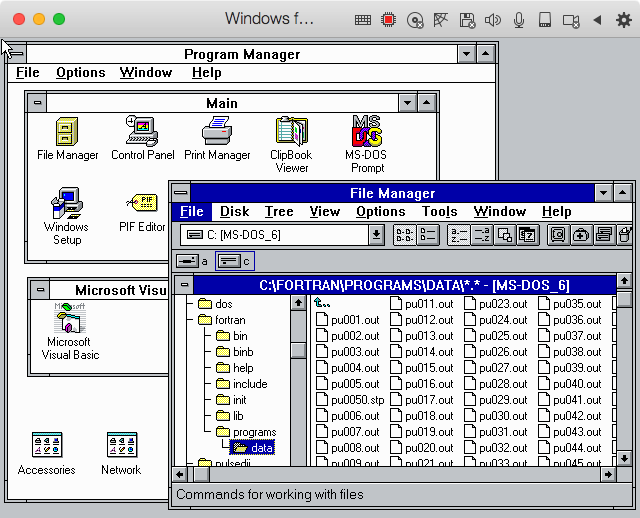
\includegraphics[width=0.75\textwidth]{windows-311.png}
	\caption{The Windows 3.11 desktop as shown in the Parallels emulator.}
	\label{fig:windows-311}
\end{figure}
%===============================================================================


Another problem to be dealt with was how to transfer the source and data files to the emulated DOS/Windows system.
I soon excluded the possibility of try to make Windows 3.11 communicate with the host OS through the network [++by setting up Windows 3.11 networking in the emulator++].
I don't even know if it can be done, but it seemed to me too much of a hassle for this simple project.
Much better is to use again a virtual floppy disk, that should be mounted alternatively (end exclusively) on macOS or on Windows 3.11. 
To create a virtual floppy disk \textsf{data.img} it is sufficient to issue the command \textsf{dd} in the macOS Terminal,

%===============================================================================
\lstset{
    language = bash,
    basicstyle = \small\bfseries\ttfamily,
    tabsize = 4,
    frame = none,
    framesep = 2em,
    framexleftmargin = 1em,
    backgroundcolor = \color{ultralightgray},
    keywordstyle = \color{darkred}\bfseries,
    morekeywords = {dd, if, of, bs, count},
    deletekeywords = {for}
}
%===============================================================================
\begin{lstlisting}
$ dd if=/dev/zero of=data.img bs=1440k count=1
\end{lstlisting}
%===============================================================================


and then run Windows 3.11 in the emulator, mount the virtual floppy disk and format it in the MS-DOS FAT format.
Using this virtual floppy disk I copied the source code of \textsf{mcphase.for} and \textsf{mcp-work.for} and the \textsf{mc-iv.dat} configuration file, transferring them in the same directories used originally.

[++ how did I find where these dirs were located??? ++]

[++ sorgente stepampl  ++] [++ già compilato, VB non è strettamente necessario il sorgente basta il binario ++]

This step completed the preparation stage of the development environment, now it was time to test how all this behaved.



\section{Running the programs}

To avoid cluttering the \textsf{mccumber/} directory containing the source files with the output data files produced by the simulations, before trying to run the two Fortran programs I create in the main project folder a new directory, \textsf{2020runs/}, copying there the \textsf{mc-iv.dat} configuration file needed to start the simulation.
[++ before: show layout of the project directory? ++]

Running \textsf{mcphase.for} is easy. In summary, all I had to do was to compile \textsf{mcphase.for}, move to the \textsf{2020runs/} directory and run the \textsf{mcphase} executable from there, as summarized below

%===============================================================================
\lstset{
    language = bash,
    basicstyle = \small\bfseries\ttfamily,
    tabsize = 4,
    frame = none,
    framesep = 2em,
    framexleftmargin = 1em,
    backgroundcolor = \color{ultralightgray},
    keywordstyle = \color{darkred}\bfseries,
    alsoletter=-,
    morekeywords = {gfortran, -cpp, -o},
    deletekeywords = {for}
}
%===============================================================================
\begin{lstlisting}
$ gfortran -cpp -Dtextout -Dsingle -o mcphase mcphase.for
$ cd ../2020runs/
$ ../mccumber/mcphase
\end{lstlisting}
%===============================================================================

obtaining at the end of the calculations a file \textsf{mc-iv.out} that contains the $I - V$ characteristic and the phase plot (for that, read below) of the junction for the set of parameters defined in \textsf{mc-iv.dat}. The calculation takes just a couple of seconds on a recent Mac, and for $\alpha_\mathrm{rf} = 0$ produces a standard non-hysteretic $I - V$ curve (Fig.~\ref{fig:mcphase-iv-single}a), while for non-zero values of $\alpha_\mathrm{rf}$ one gets the standard staircase-like $I - V$ curves with the rf-induced current steps (Fig.~\ref{fig:mcphase-iv-single}b and Fig.~\ref{fig:mcphase-iv-single}c).

%===============================================================================
\begin{figure}[h]
{
	\fboxsep=0pt
	\mbox{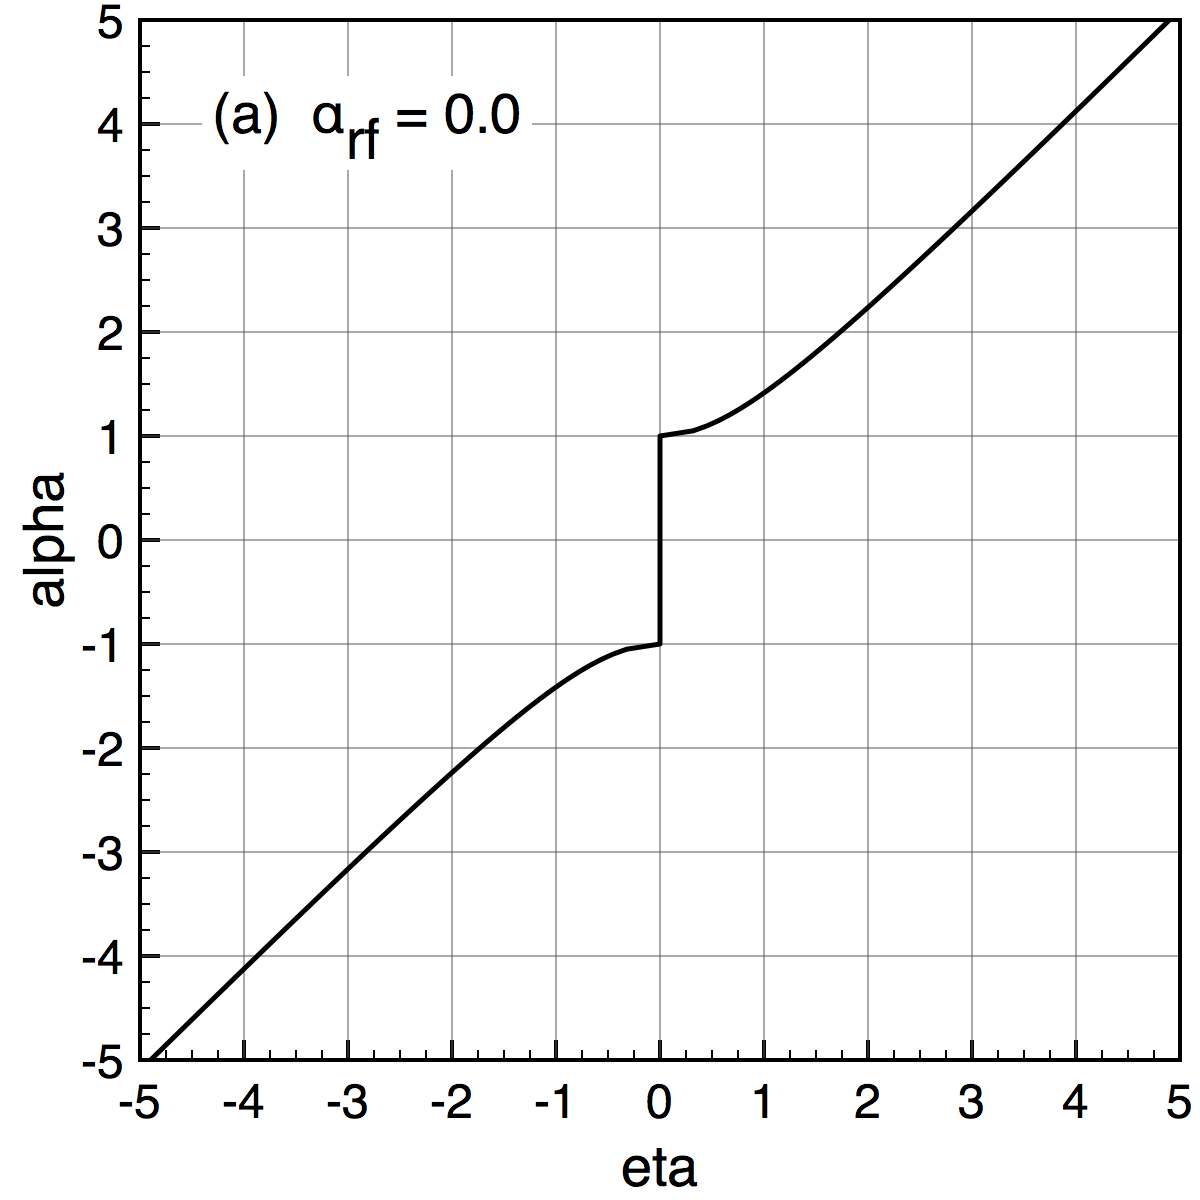
\includegraphics[width=0.325\textwidth]{mcphase-iv-single-alpharf0.png}}
	\hfill
	\mbox{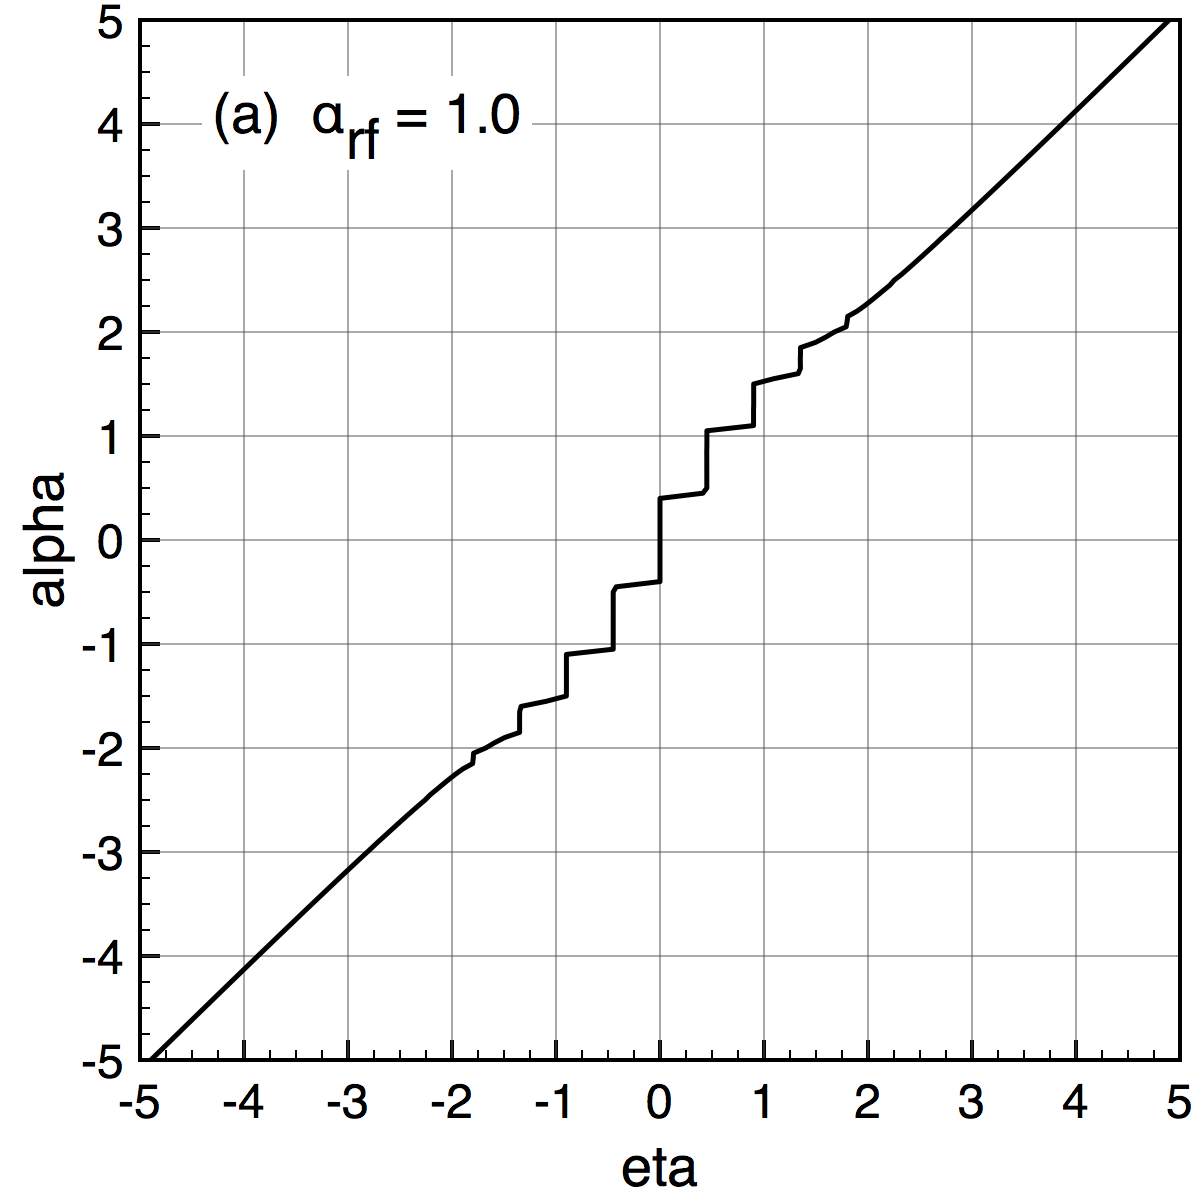
\includegraphics[width=0.325\textwidth]{mcphase-iv-single-alpharf1.png}}
	\hfill
	\mbox{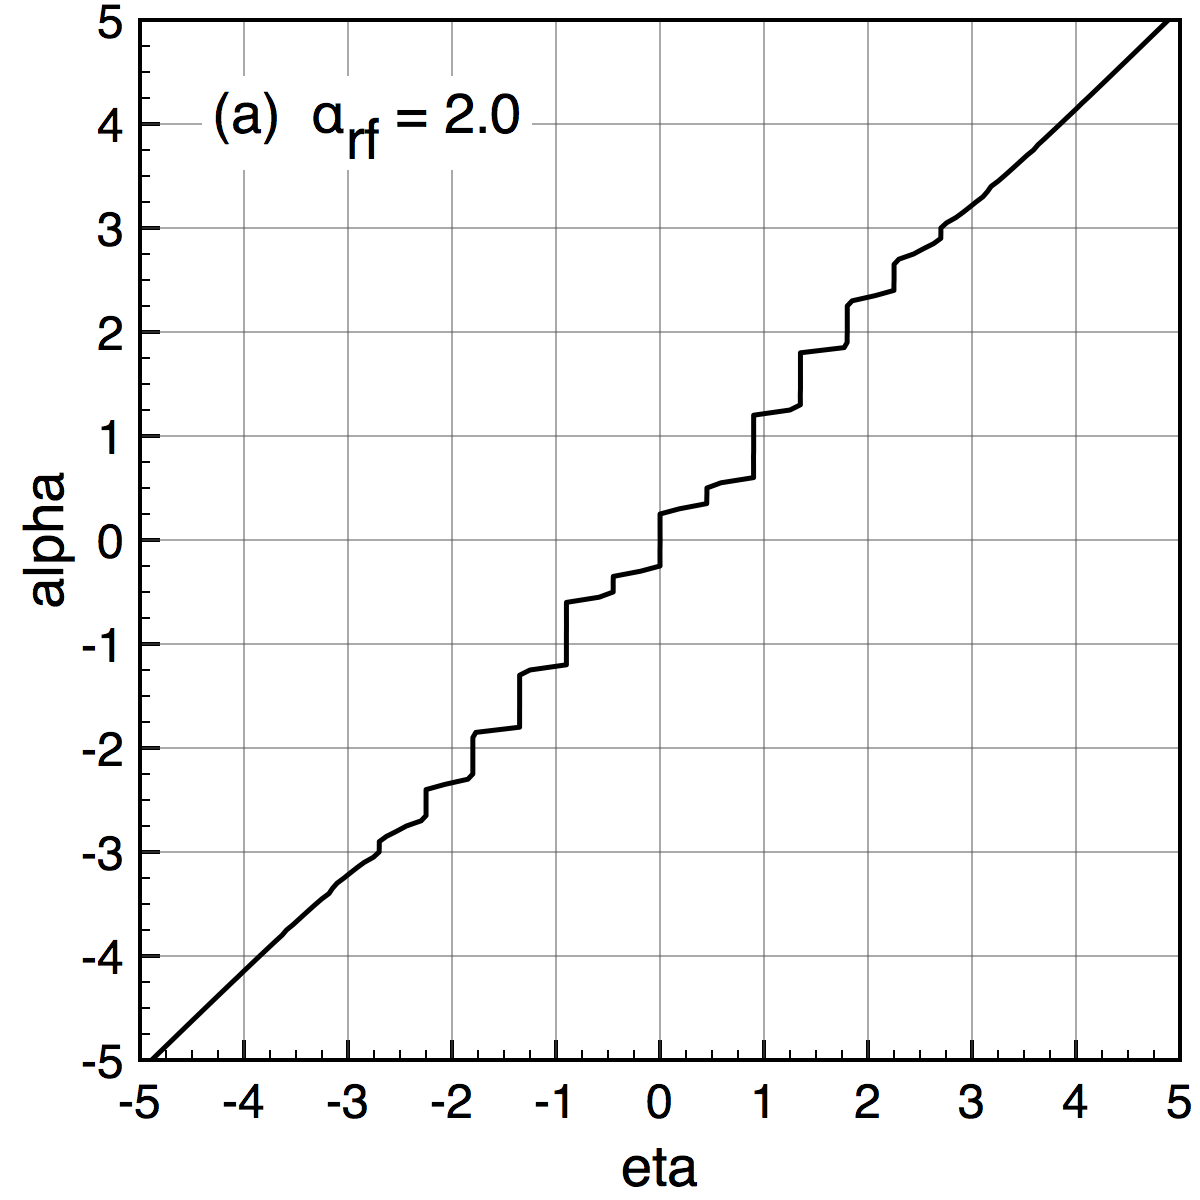
\includegraphics[width=0.325\textwidth]{mcphase-iv-single-alpharf2.png}}
}
	\caption{$I - V$ characteristics of a junction with $\beta_c = 0.01$, driven by a sinusoidal rf drive of frequency $\Omega = 0.45$ and (a) $\alpha_\mathrm{rf} = 0.0$, (b) $\alpha_\mathrm{rf} = 1.0$ and (c) $\alpha_\mathrm{rf} = 2.0$. The rf-induced current steps are clearly visible when $\alpha_\mathrm{rf} > 0$.}
	\label{fig:mcphase-iv-single}
\end{figure}
%===============================================================================


To simulate a pulsed rf drive, it is sufficient to compile \textsf{mcphase.for} with the \textsf{-Dpulsed} switch and rerun the simulation (Fig.~\ref{fig:mcphase-iv-pulsed}). The Figure shows clearly that with the pulsed rf drive there are fewer but much larger rf-induced steps and that they can be nearly as wide as the critical current for $\alpha_\mathrm{rf} = 0.0$ (compare Fig.~\ref{fig:mcphase-iv-pulsed}a) and (Fig.~\ref{fig:mcphase-iv-pulsed}c).

%%===============================================================================
%\begin{lstlisting}
%$ gfortran -cpp -Dtextout Dpulsed -o mcphase mcphase.for
%$ cd ../2020runs/
%$ ../mccumber/mcphase
%\end{lstlisting}
%%===============================================================================

%===============================================================================
\begin{figure}[h]
{
	\fboxsep=0pt
	\mbox{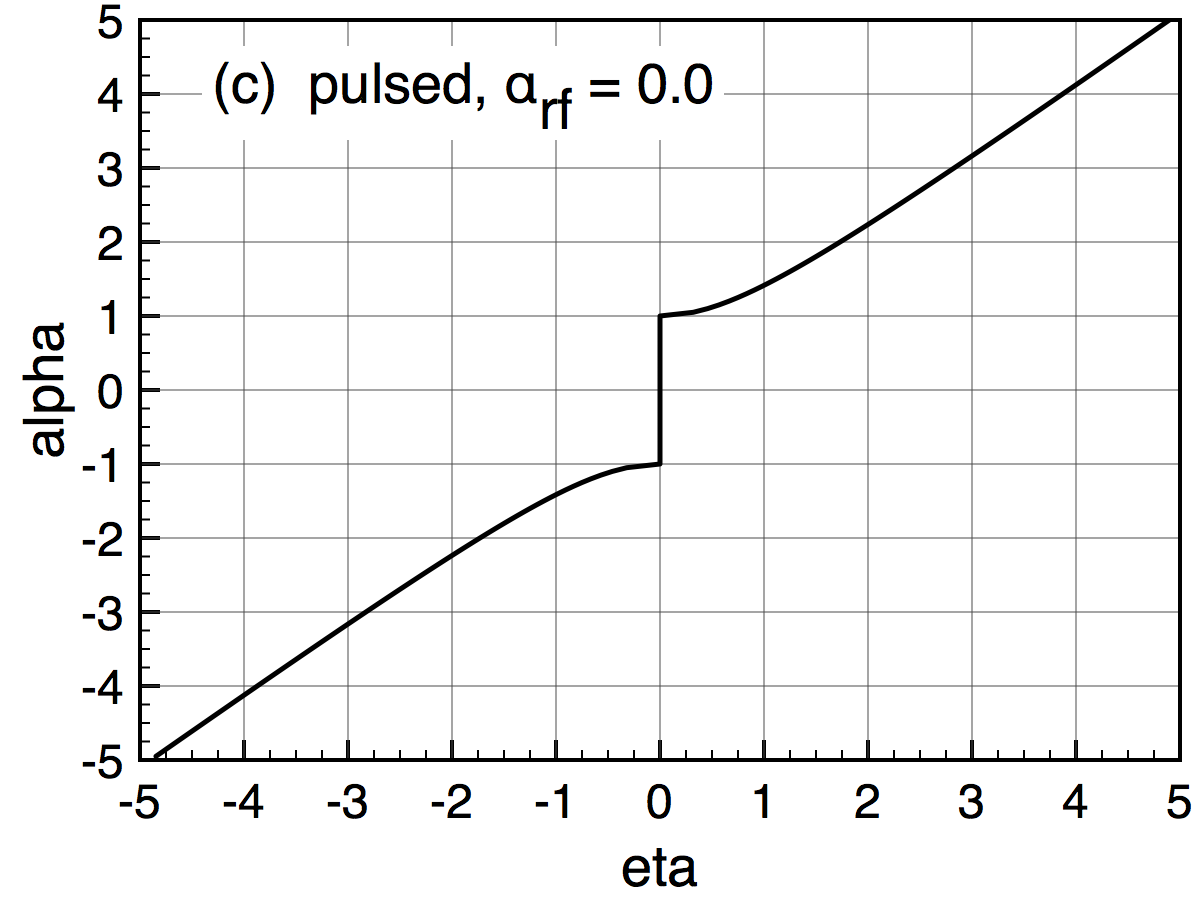
\includegraphics[width=0.325\textwidth]{mcphase-iv-pulsed-alpharf0.png}}
	\hfill
	\mbox{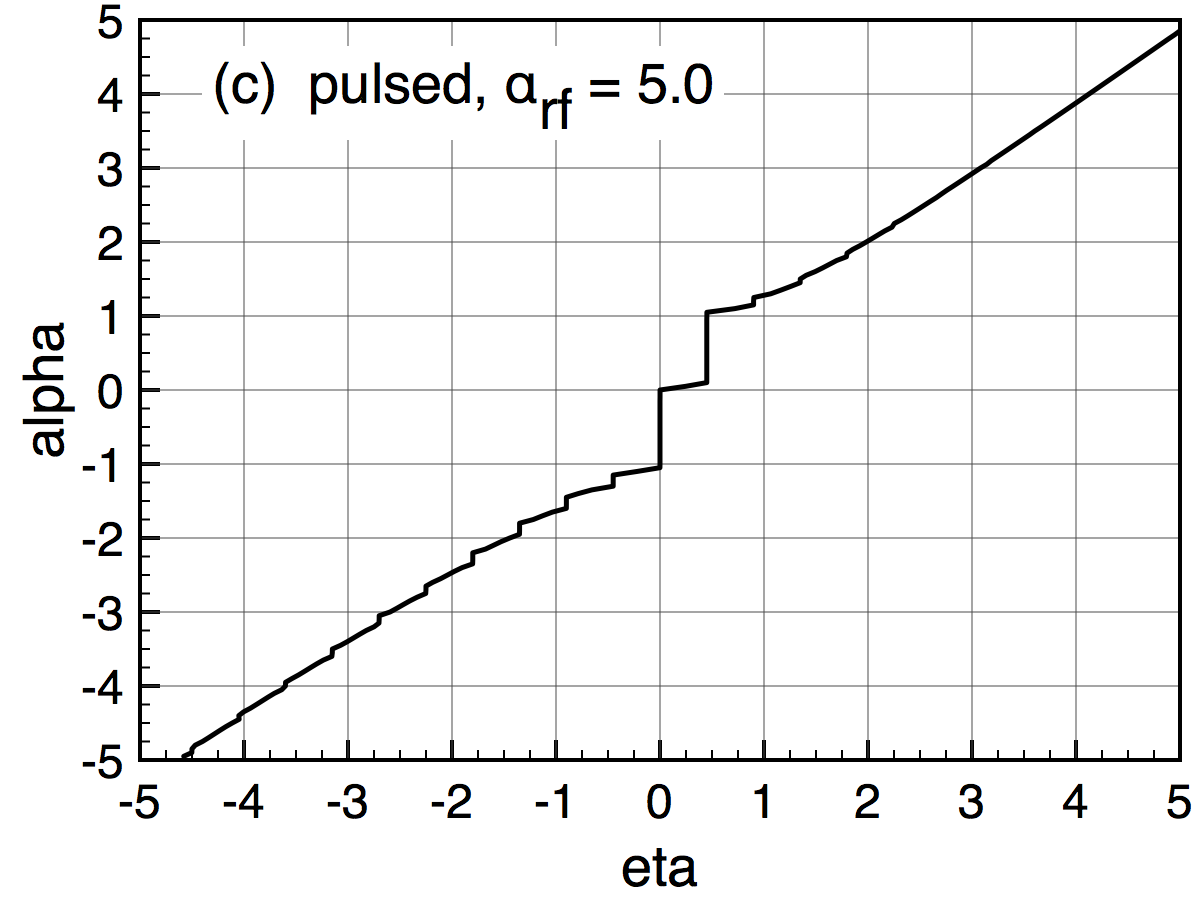
\includegraphics[width=0.325\textwidth]{mcphase-iv-pulsed-alpharf5.png}}
	\hfill
	\mbox{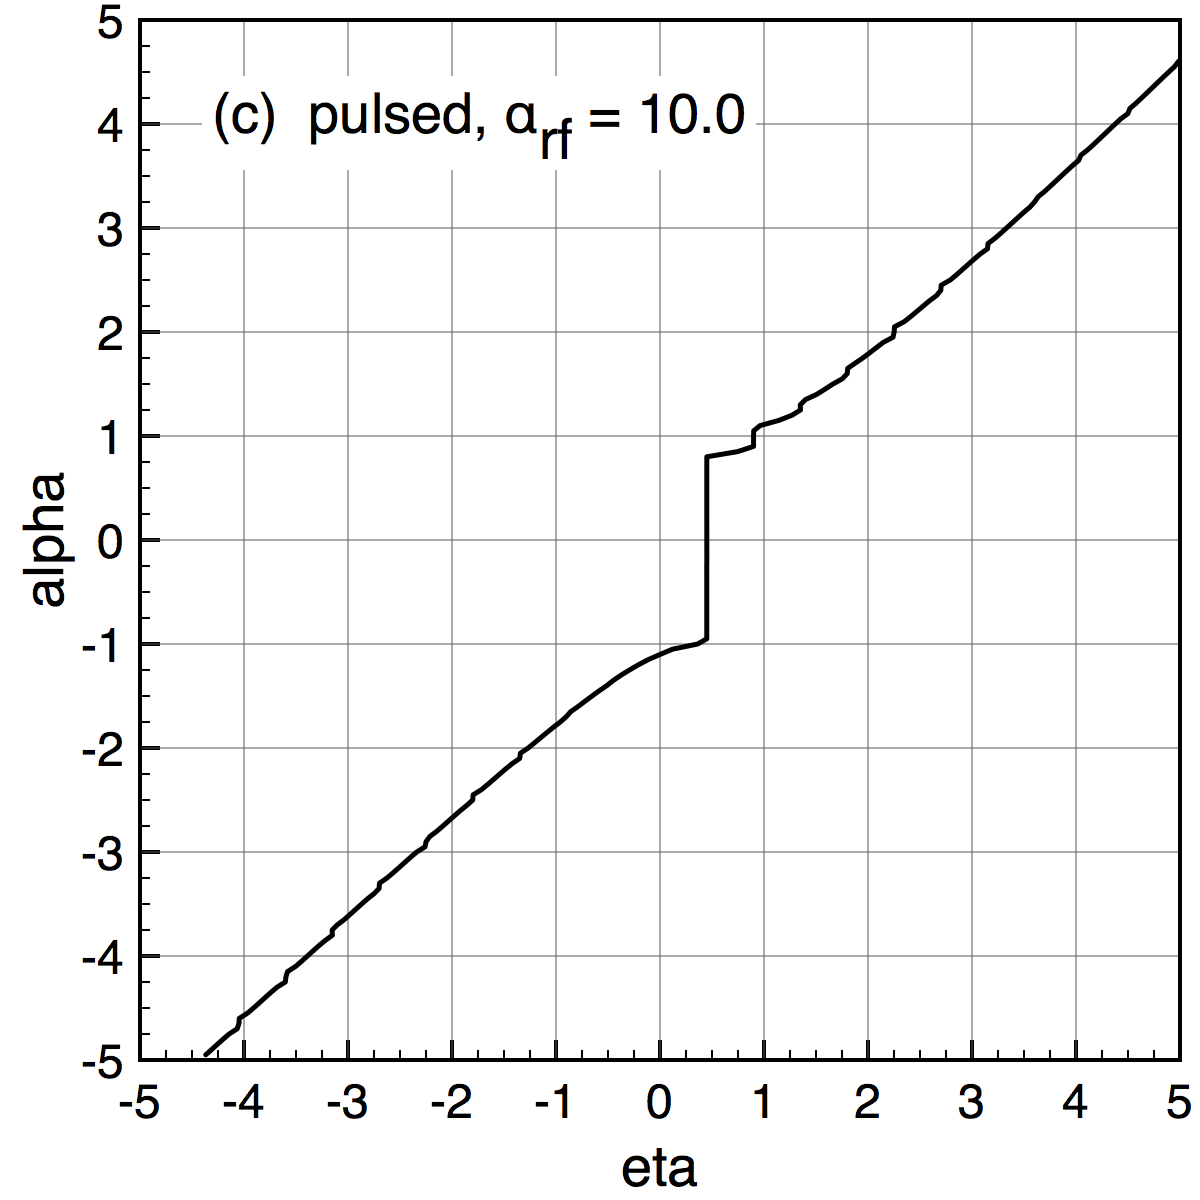
\includegraphics[width=0.325\textwidth]{mcphase-iv-pulsed-alpharf10.png}}
}
	\caption{$I - V$ characteristics of a junction with $\beta_c = 0.01$, driven by a pulsed rf drive of frequency $\Omega = 0.45$ for: (a) $\alpha_\mathrm{rf} = 0.0$, (b) $\alpha_\mathrm{rf} = 5.0$ and (c) $\alpha_\mathrm{rf} = 10.0$. For $\alpha_\mathrm{rf} > 0$ the rf-induced steps are much larger than with the standard sinusoidal rf-drive.}
	\label{fig:mcphase-iv-pulsed}
\end{figure}
%===============================================================================


The second Fortran program, \textsf{mcp-work.for}, is much more interesting. While \textsf{mcphase.for} can calculate the $I - V$ characteristic of the junction for a single value of $\alpha_\mathrm{rf}$ and for increasing or decreasing values of the normalized current $\alpha_\mathrm{dc}$, \textsf{mcp-work.for} automatically sweeps the normalized current $\alpha_\mathrm{dc}$ in both directions to help visualize better the possible hysteresis of the junction and calculates the $I - V$ characteristics for a range of values of $\alpha_\mathrm{rf}$, saving each curve in a separate output file. Unfortunately, the lower and upper limits and the step size of $\alpha_\mathrm{rf}$ are hardcoded in the Fortran source code ad every change requires a recompilation of \textsf{mcp-work.for} (a minor hassle, as the compilation takes just a couple of seconds on a modern machine).


Running \textsf{mcp-work.for} is very similar to the previous case. First, it is necessary to compile \textsf{mcp-work.for} with the proper compiler switches, then one moves to \textsf{2020runs/} directory and runs the \textsf{mcp-work} executable from there. The whole process is summarized below for the standard sinusoidal drive,

%===============================================================================
\lstset{
    language = bash,
    basicstyle = \small\bfseries\ttfamily,
    tabsize = 4,
    frame = none,
    framesep = 2em,
    framexleftmargin = 1em,
    backgroundcolor = \color{ultralightgray},
    keywordstyle = \color{darkred}\bfseries,
    alsoletter=-,
    morekeywords = {gfortran},
    deletekeywords = {for}
}
%===============================================================================
\begin{lstlisting}
$ gfortran -cpp -Dtextout -Dsingle -o mcp-work mcp-work.for
$ cd ../2020runs/
$ ../mccumber/mcp-work
\end{lstlisting}
%===============================================================================

while the only modification needed to perform calculations using the pulsed drive is to change the \textsf{-Dsingle} switch to \textsf{-Dpulsed}, 

%===============================================================================
\begin{lstlisting}
$ gfortran -cpp -Dtextout -Dpulsed -o mcp-work mcp-work.for
$ cd ../2020runs/
$ ../mccumber/mcp-work
\end{lstlisting}
%===============================================================================

Also the names of the output files are hard-coded in the \textsf{mcp-work.for} in the \textsf{filewrite} variable and are conventionally composed by a two-letter prefix ("SI" for the single drive, "BI" for the biharmonic driva and "PU" for the pulsed drive) followed by a tree-digit integer containing the cycle number (see Section~\ref{compilation-with-gfortran}).

On a modern machine the whole calculation with $100$ $\alpha_\mathrm{rf}$ steps takes around $2 - 4$ minutes and most of the time is spent printing the calculated $I - V$ curves for each value of $\alpha_\mathrm{rf}$. Such feedback was necessary at the time of the original calculation, as every new calculated point of the $I - V$ curves appeared on the screen after several minutes, now the results literally flow on the screen at a speed that makes them almost illegible.

The output files should be transferred to the Windows 3.11 virtual machine to be processed by \textsf{stepampl}, the Visual Basic application described in Section~\ref{visual-basic-code}. However Windows 3.11 does not \emph{understand} UNIX line terminators and cannot read the output files without a proper line terminator conversion. This conversion can be easily done in the macOS Terminal with the following command

%===============================================================================
\lstset{
    language = bash,
    basicstyle = \small\bfseries\ttfamily,
    tabsize = 4,
    frame = none,
    framesep = 2em,
    framexleftmargin = 1em,
    backgroundcolor = \color{ultralightgray},
    keywordstyle = \color{darkred}\bfseries,
    alsoletter=;,
    morekeywords = {;},
}
%===============================================================================
\begin{lstlisting}
$ for f in $(ls *.out); do sed -i .bak s/$/$'\r'/ $f ; done
\end{lstlisting}
%===============================================================================

that converts the line terminators of all the \textsf{.out} output files from the UNIX format containing only a line-feed (LF) to the carriage return followed by a line-feed (CRLF) format used by all versions of Microsoft Windows (slightly different versions of the command can be usually found on internet; however the format used above is POSIX-compliant and should run on all UNIX flavours). The \textsf{-i} switch allows in-place conversion of each files (the original files are saved with the \textsf{.bak} extension and can be easily removed after the conversion).

Now the output files in the proper Windows format can be transferred onto the virtual floppy disk image. %virtual floppy disk image can be mounted on the Desktop of the host operating system by double-clicking on its icon and the output files in the proper Windows format can be transferred onto the virtual floppy disk. 
When the transfer is done, the floppy disk image must be unmounted from the Desktop of the host operating system and mounted in the emulator. This allows to open the floppy disk in Windows 3.11 so that the output files can be copied in an (preferably) empty directory of Windows 3.11. 
Now it is the time to run the Visual Basic application, either by running the precompiled \textsf{stepampl.exe} application or by opening the Visual Basic project and running the program form there (Fig.~\ref{fig:stepampl}). [++ 100 data files max ++] 
The summary file containing the the size of the quantized current steps for a single simulation are saved in a file with extension \textsf{.STP} (for steps) and can be transferred to the host operating system via the floppy disk image.

%===============================================================================
\begin{figure}[tbh]
	\centering
	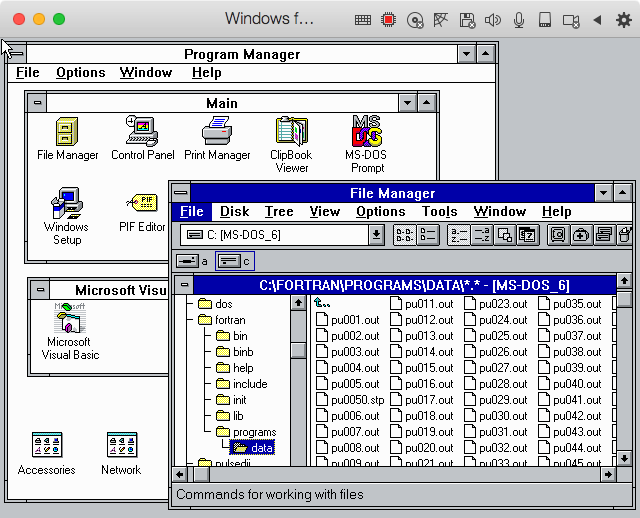
\includegraphics[width=0.75\textwidth]{windows-311.png}
	\caption{Windows 3.11 desktop showing the program \textsf{stepampl} that has just finished to process the data files.}
	\label{fig:stepampl}
\end{figure}
%===============================================================================

At the time of writing the original paper \cite{Maggi:1996}, the whole process had to be repeated each night for a different set of input parameters,  or for a different kind of rf drive (single, biharmonic or pulsed). As noted above (Section~\ref{computational-context}), as each night I had four DEC machines  available, I could use three of them to simulate in parallel the junction behaviour with the pulsed drive with three different values of the (normalized) width of the pulse signal, $\rho$, while keeping constant all the other junction parameters, such $\beta$ and $\Omega$.
The only thing that in different in the three simulation is the range over which to change $\alpha_\mathrm{rf}$, which depends on the value of $\rho$ (shorter pulses require a much larger intensity of the rf-signal to have the same effect on the junction)

The fourth machine was reserved to simulate the junction behaviour with the standard sinusoidal drive, using exactly the same set of junction parameters.
Each night a different set of junction parameters was used.

Luckily the original paper  contained all the information needed to reproduce the results shown in the figures, without having to repeat the whole analysis from scratch. The parameters used in all runs were: hysteresis parameter $\beta = 0.01$, frequency of the sinusoidal or pulsed  rf signal $\Omega = 0.45$, normalized current bias ranging between $\alpha_\mathrm{dc} = -5.0$ and $\alpha_\mathrm{dc} = 5.0$, integration time $\tau = 500$, step $\Delta \tau = 0.01$. For the simulation with the sinusoidal drive, 
the amplitude of the rf signal$\alpha_\mathrm{rf}$ was varied between $0.0$ and $5.0$, with a step $\Delta \alpha_\mathrm{rf} = 0.1$. 
The three simulations with the pulsed drive were done using: 
(1) pulse width $\rho = 0.250$ and $\alpha_\mathrm{rf} = 0.0, 0.1, ... 10.0$;
(2) pulse width $\rho = 0.125$ and $\alpha_\mathrm{rf} = 0.0, 0.2, ... 20.0$;
(3) pulse width $\rho = 0.050$ and $\alpha_\mathrm{rf} = 0.0, 0.5, ... 50.0$.

The resulting output and summary files are saved in separate folders in the \textsf{2020runs/} directory, named \textsf{SINGLE/}, \textsf{PULS0250}, \textsf{PULS125}, \textsf{PULS0050} after their DOS counterparts.

To reproduce the first and second figure of \cite{Maggi:1996} I made the only concession to modernity and, instead of trying to recreate them with the original plotting program used originally, probably \textsf{Origin 2.0},\footnote{https://www.originlab.com} I decided to write a couple of small R scripts that could automate the task.
The results are shown in Fig.~\ref{fig:step-width} and Fig.~\ref{fig:pulsed-ivs} and, as expected, are identical to those reported in the first two figures of \cite{Maggi:1996}. Figure 3 of the original paper coulb be trivially reproduced by plotting the maxima of the curves of Fig.~\ref{fig:step-width} ($\Delta i_n$ vs. $\alpha_\mathrm{rf}$ for the four different cases considered here.


%%===============================================================================
%\begin{figure}[h]
%{
%	\fboxsep=0pt
%	\mbox{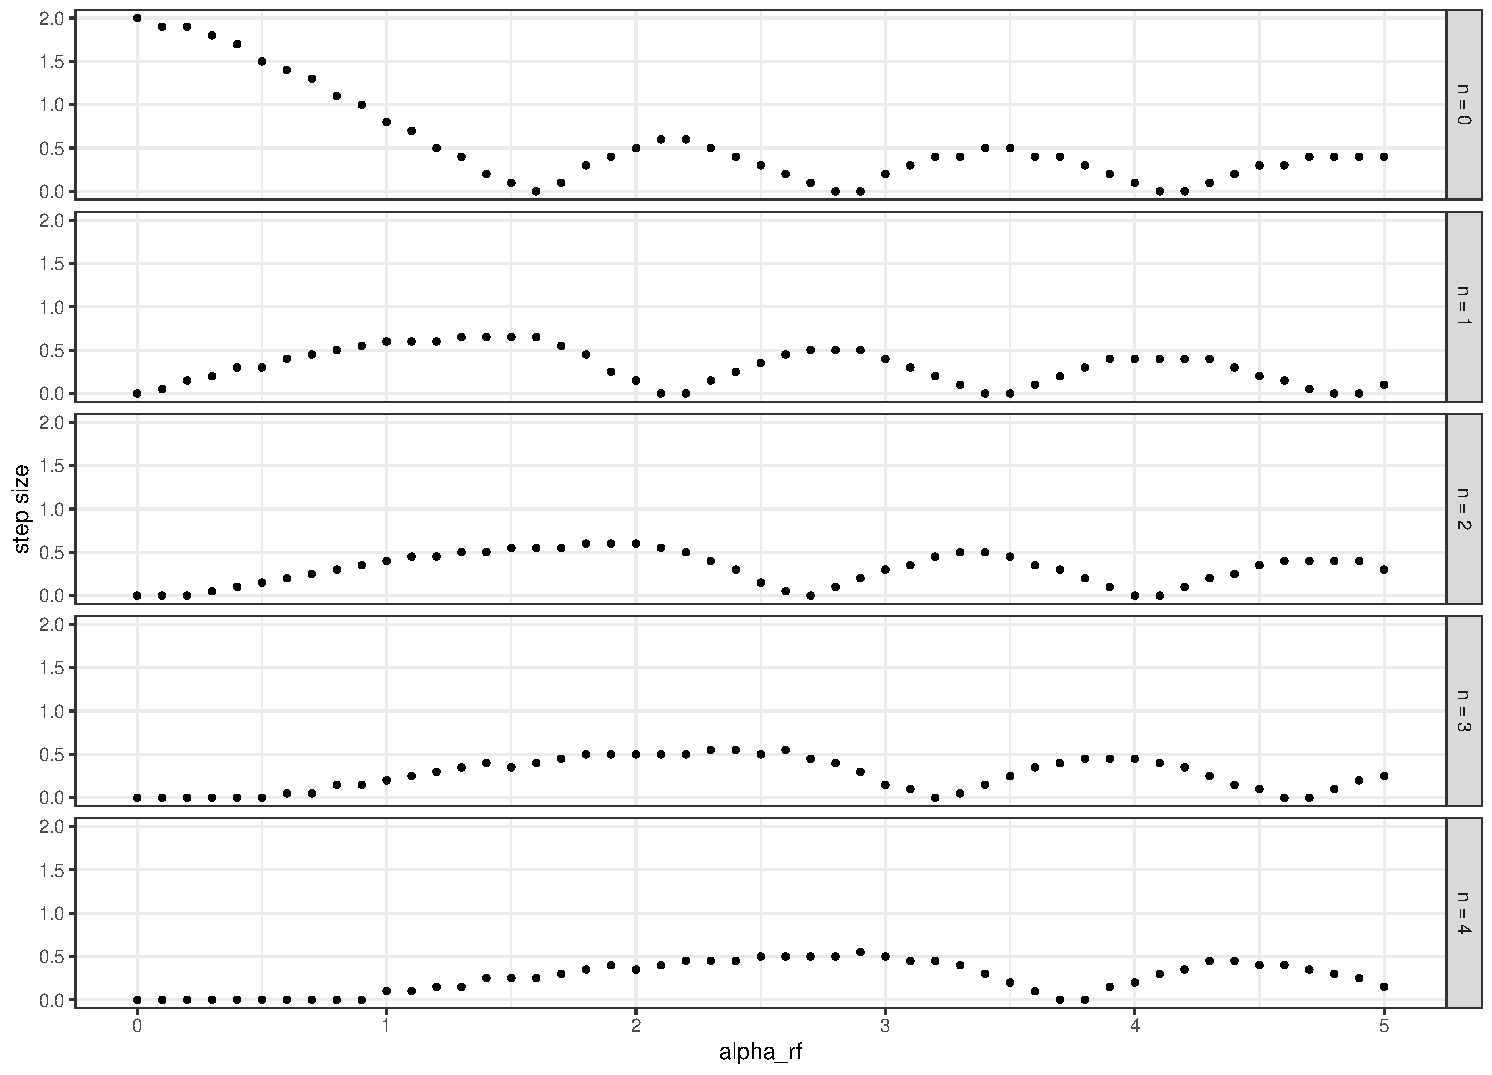
\includegraphics[width=0.45\textwidth]{SINGLE.pdf}}
%	\hfill
%	\mbox{\includegraphics[width=0.45\textwidth]PULS0250.pdf}}
%}
%%{
%%	\fboxsep=0pt
%%	\mbox{\includegraphics[width=0.45\textwidth]PULS0250.pdf}}
%%	\hfill
%%	\mbox{\includegraphics[width=0.45\textwidth]PULS0050.pdf}}
%%}
%	\caption{.}
%	\label{fig:step-width}
%\end{figure}
%%===============================================================================
%===============================================================================
\begin{figure}[tbh]
	\centering
	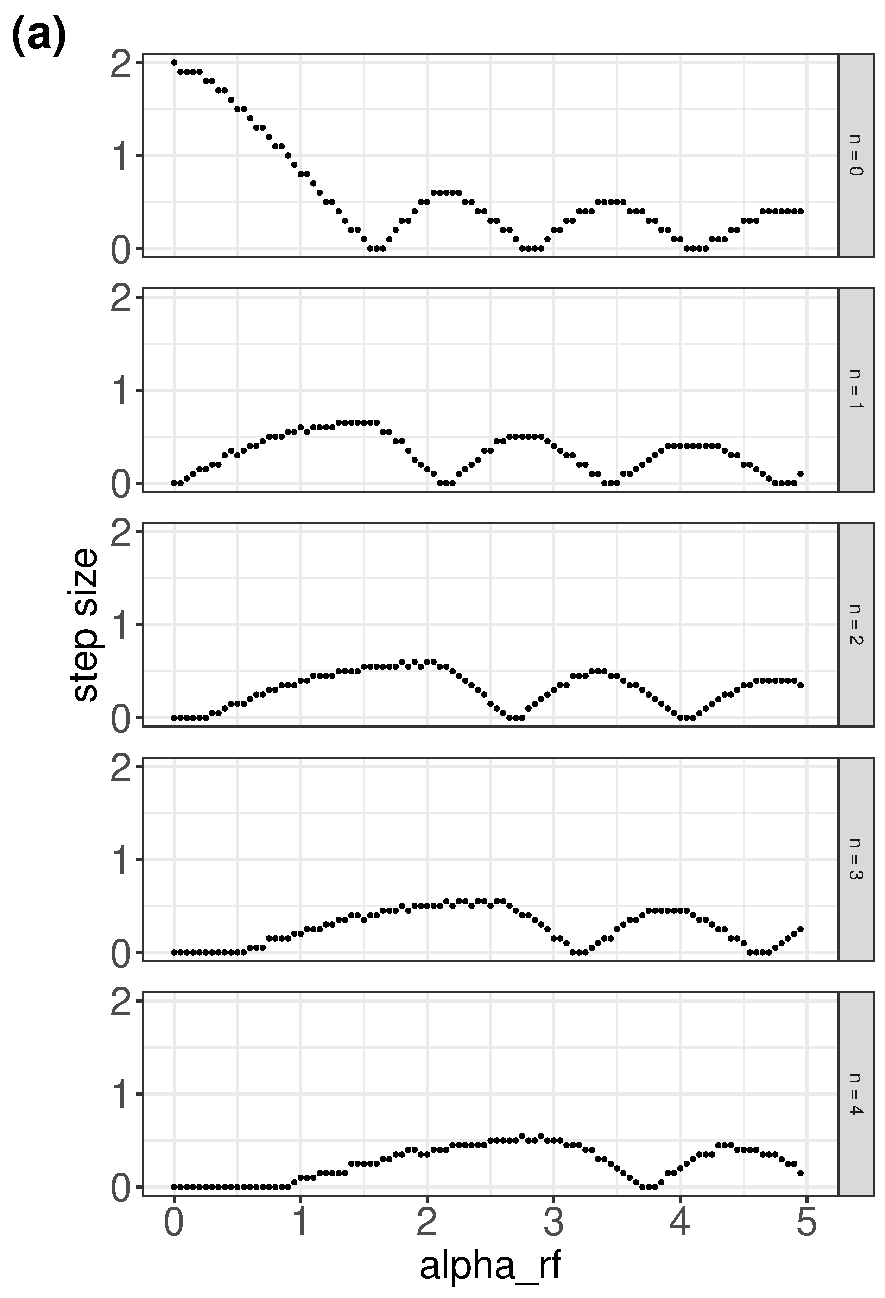
\includegraphics[width=0.45\textwidth]{SINGLE2.pdf}
	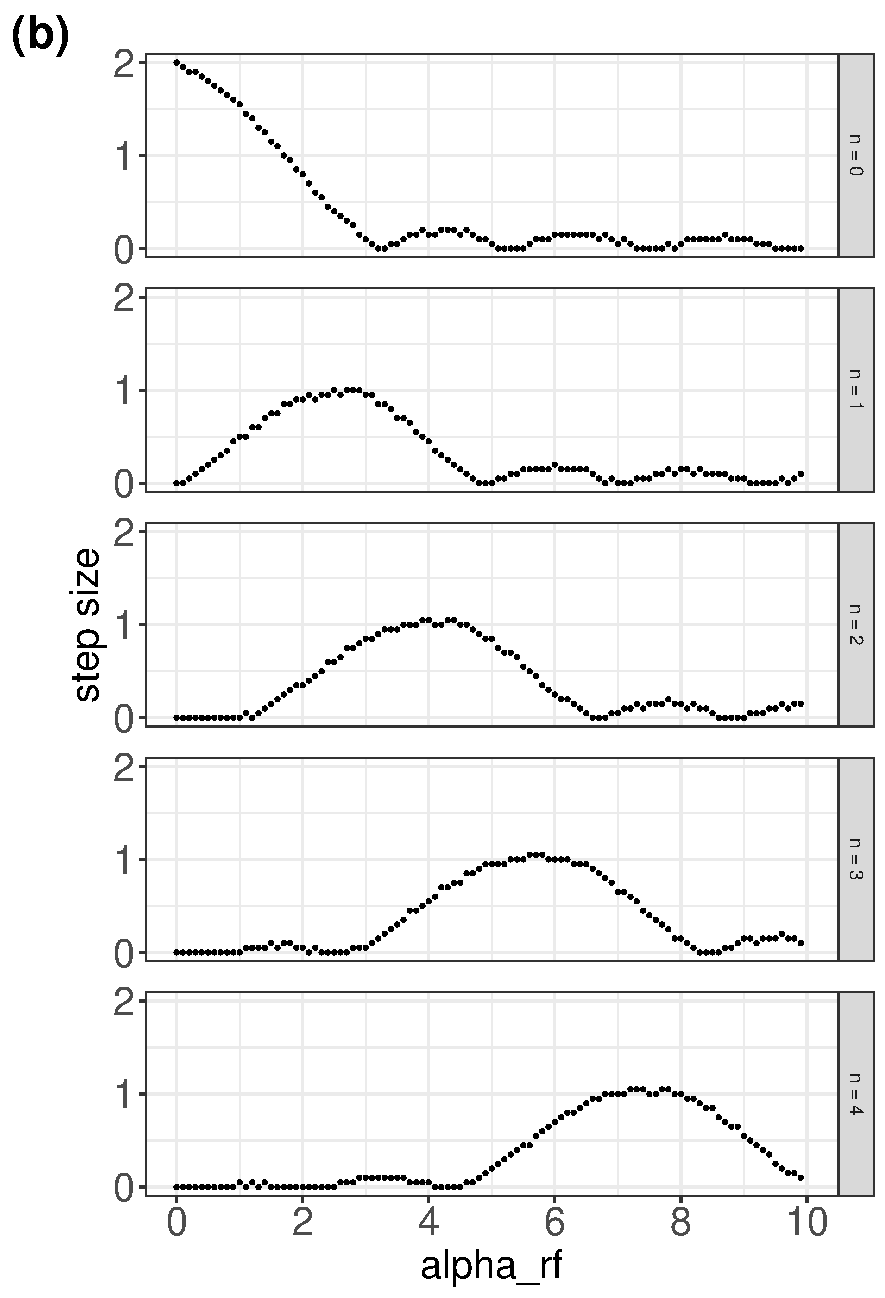
\includegraphics[width=0.45\textwidth]{PULS0250.pdf}
	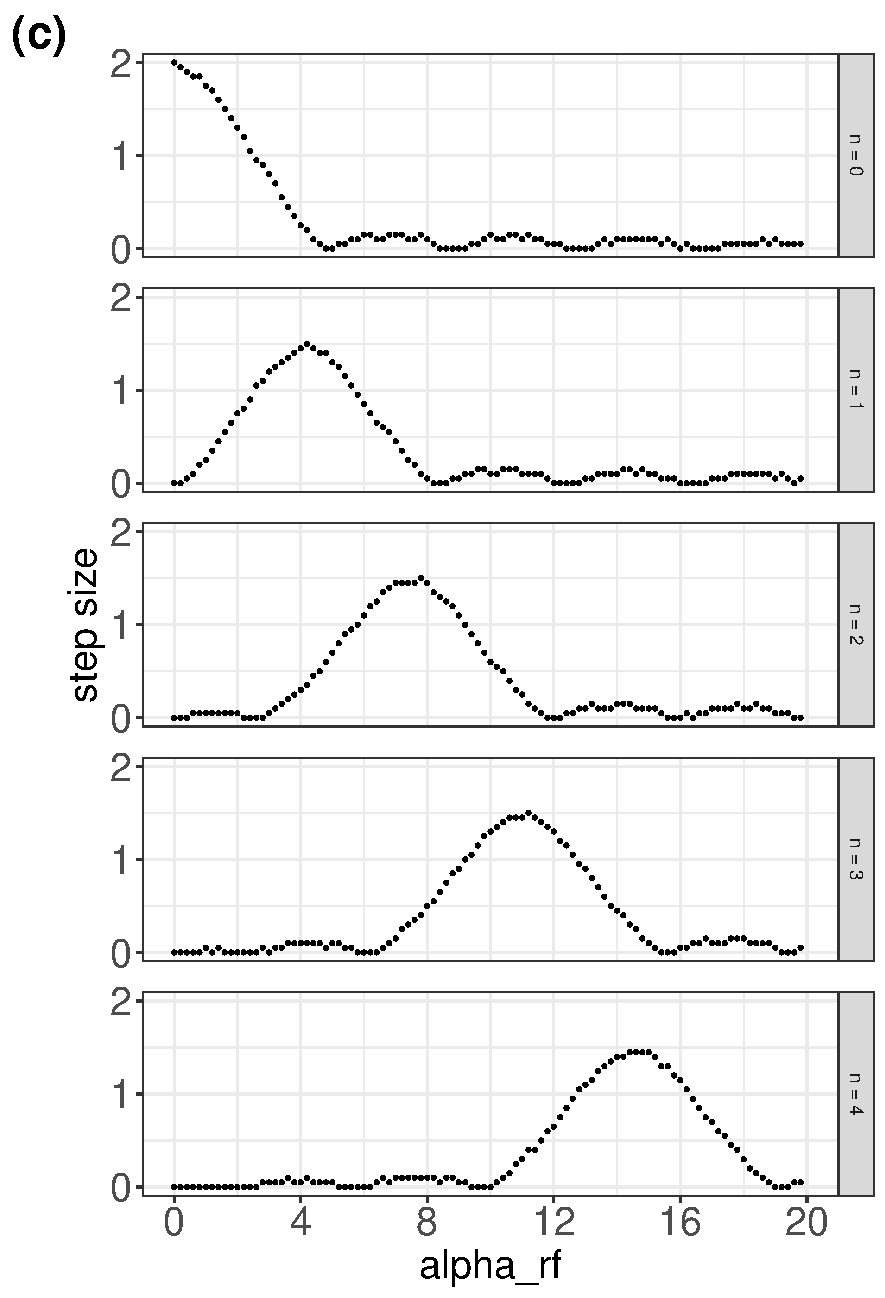
\includegraphics[width=0.45\textwidth]{PULS0125.pdf}
	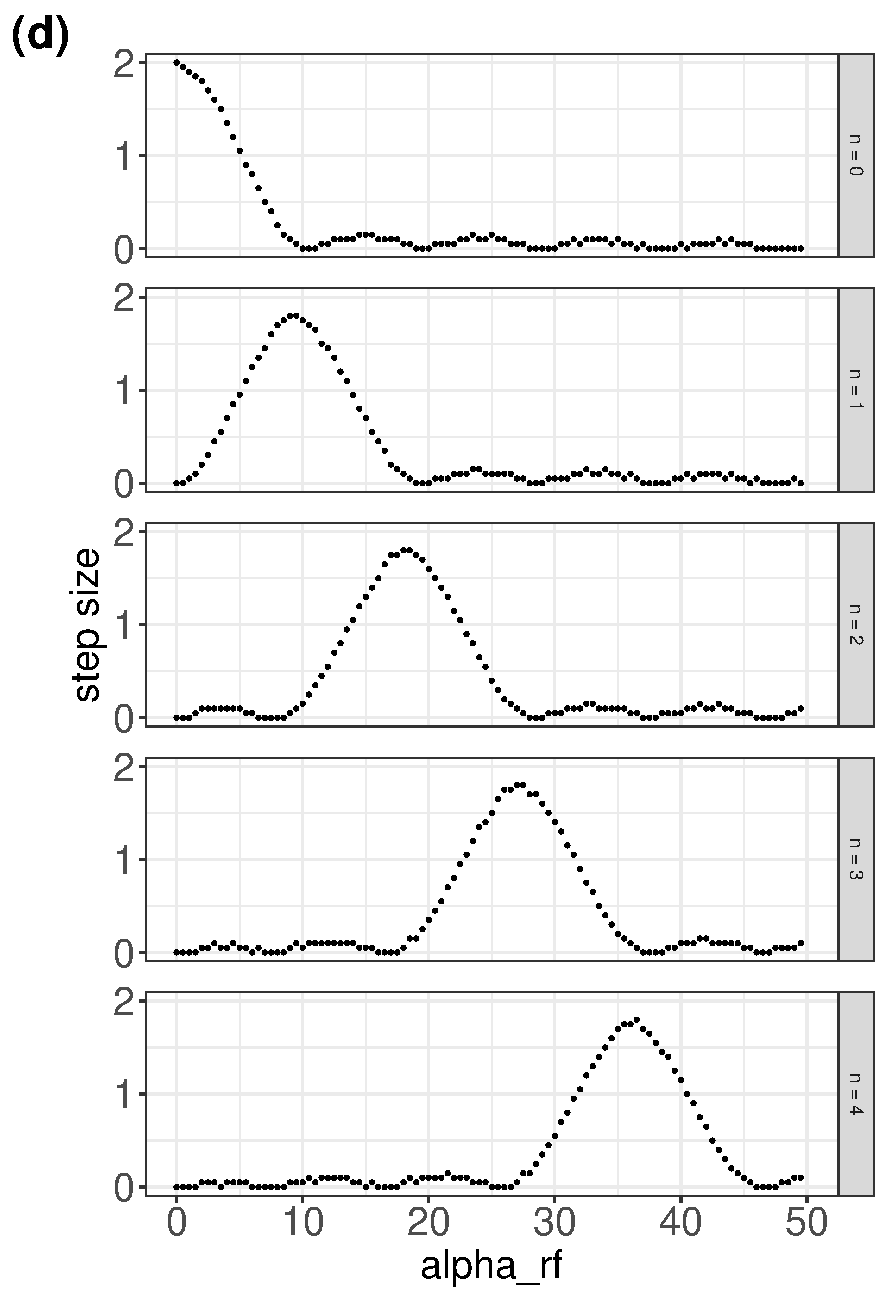
\includegraphics[width=0.45\textwidth]{PULS0050.pdf}
	\caption{Dependence of the step size $\Delta i_n$ on the amplitude of  $\alpha_\mathrm{rf}$, for $n = 0. . . 4$. The $n = 0$ step is the normalized total critical current $\Delta i_0$ of the junction. The junction parameters are $\beta = 0. 01$ and $\Omega = 0. 45$; (a) sinusoidal drive, (b) pulsed drive with $\rho = 0. 250$, (c) pulsed drive with $\rho = 0. 125$, (d) pulsed drive with $\rho = 0. 050$.}
	\label{fig:step-width}
\end{figure}
%===============================================================================

%===============================================================================
\begin{figure}[tbh]
	\centering
	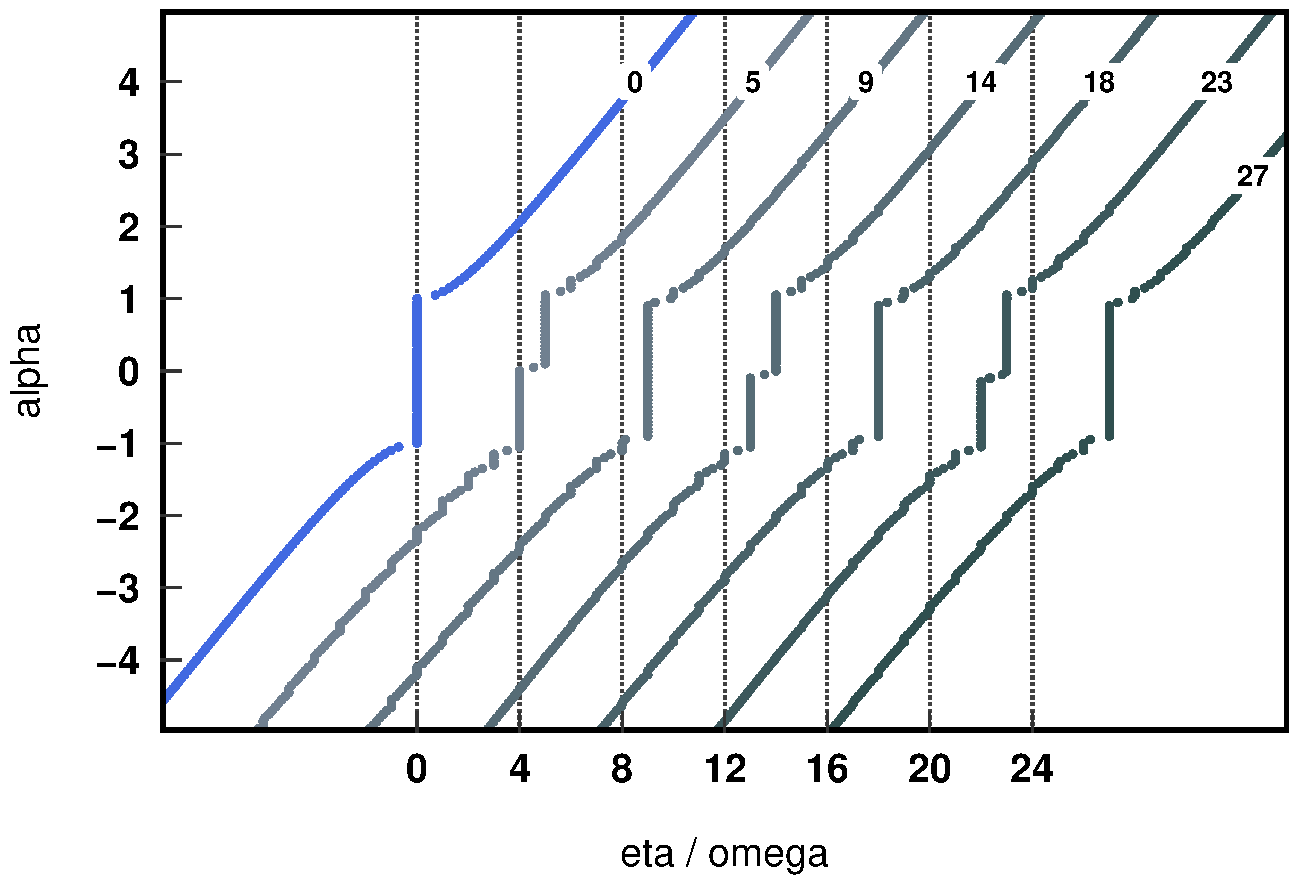
\includegraphics[width=0.45\textwidth]{PULS0050-IV.pdf}
	\caption{$I - V$ curves of a junction with $\beta = 0.01$ for several values of the rf bias. The junction is  irradiated by a train of rf pulses of repetition frequency $\Omega = 0.45$ and pulse duration $\rho = 0.05$. Each curve has been offset by $4 \Omega$. The vertical dotted lines mark the position of the zero-voltage axis for the $I - V$ curve located immediately to the right.}
	\label{fig:pulsed-ivs}
\end{figure}
%===============================================================================


Similar considerations can be made for the reproduction of Figure 4, which considers a slightly hysteretic junction with $\beta = 1.0$. In the spirit of this challenge I have chosen to show instead [++ the $I - V$ curves of the simulated junction with $\beta = 1.0$ and ++] the related $\Delta i_n$ vs. $\alpha_\mathrm{rf}$ curves for the two most significant cases of rf drive, i.e., the sinusoidal drive and the pulsed drive with $\rho = 0.050$ (Fig.~\ref{fig:step-width-beta1}).

%===============================================================================
\begin{figure}[tbh]
	\centering
	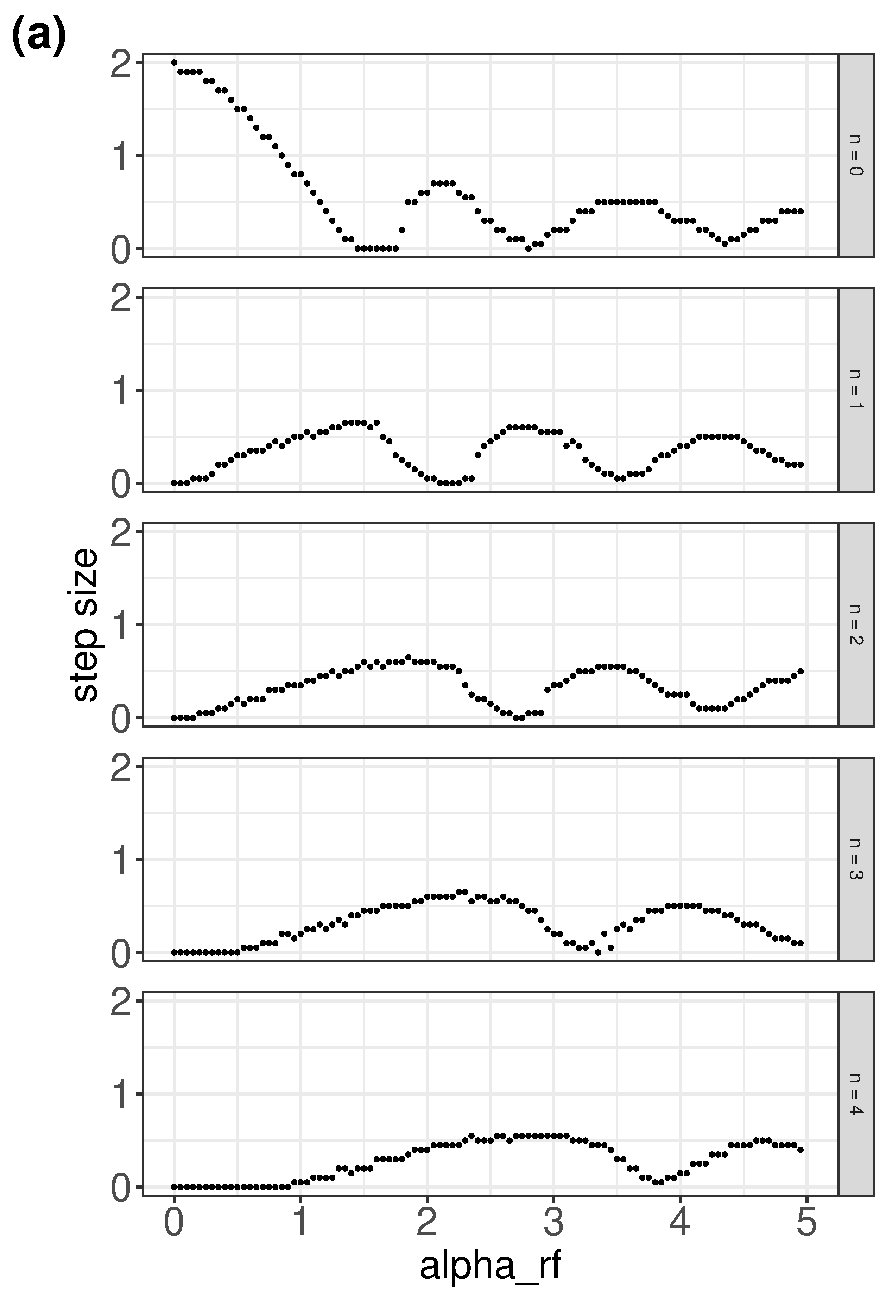
\includegraphics[width=0.45\textwidth]{SINGLE-BETA1.pdf}
	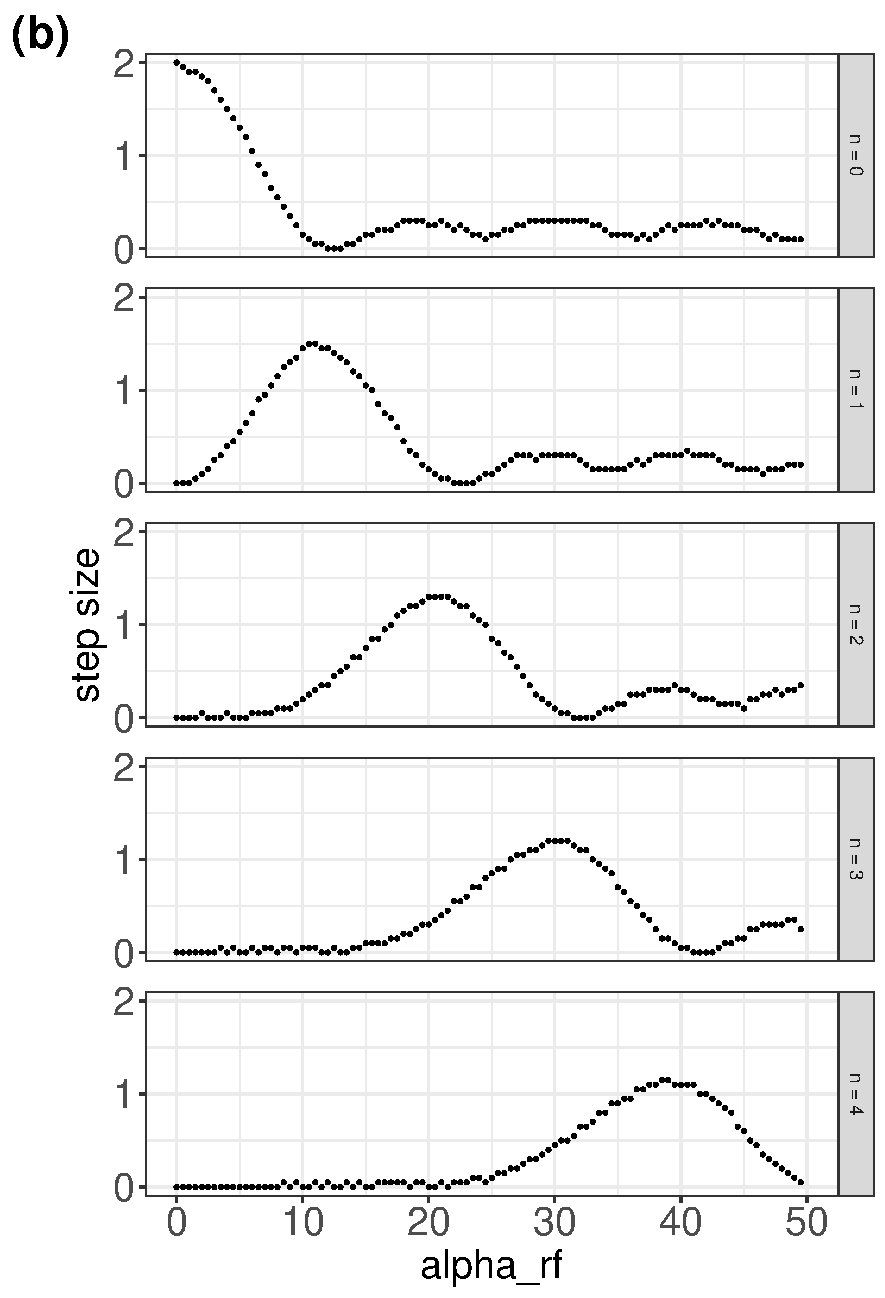
\includegraphics[width=0.45\textwidth]{PULS0050-BETA1.pdf}
	\caption{Dependence of the step size $\Delta i_n$ on the amplitude of  $\alpha_\mathrm{rf}$, for $n = 0. . . 4$. The $n = 0$ step is the normalized total critical current $\Delta i_0$ of the junction. The junction parameters are $\beta = 1.0$ and $\Omega = 0. 45$; (a) sinusoidal drive, (b) pulsed drive with $\rho = 0. 050$.}
	\label{fig:step-width-beta1}
\end{figure}
%===============================================================================





\section{Discussion}

If I would start the project today from scratch I think I would handle things quite differently:

\begin{enumerate}

\item Use Python instead of Fortran. Fortran, despite its venerable age, is stil an excellent language for scientific programming, but Python is much more comfortable to use, and the availability of excellent libraries such as NumPy and SciPy and of Fortran and C bindings to enhance performance in time-critical sections of code, make it the best tool today for numerical computations.

\item Do not use Visual Basic. First of all I would avoid the use a new language, as was Visual Basic 1.0 at the time. In 1993-94 it would have been very hard to foresee the rapid demise of Microsoft's Visual Basic, exactly as it would have been impossible to foresee the explosive success of Python, but in any case using a language only when it is stable, runs on a wide array of operating systems and is accepted by a wide community of developers is a safe bet.
[++ The same can be said today for Apple's Swift, until the language does not support Windows as well as macOS and Linux and it is not used by a large community outside that of Apple developers, I would never use it for a (serious) (research) project].

\end{enumerate}
 

\section{Conclusions}

Going back to this old paper has been an exceptionally interesting experience and I must thank the organizers of this challenge for the opportunity offered.

%literally invent the data in their papers.
However this is not only a nostalgic attitude. The reproducibility or replicability crisis is a serious issue today \cite{Miyakawa:2020}, when many scientific studies are difficult to reproduce or replicate and  true science is challenged daily by cheaters that publish papers with fabricated, falsified, or modified data or results.

Being able to go back and redo what has been done in the past assures that...

[++ SUPPLEMENYTARY INFO??? ++]



%===============================================================================
%Among the things that might be interesting is:
%
%How did you conserve the sources
%Did you take care of registering RNG seed (if you use it)
%Did you save command line options (if you need some options)
%Did you need to adapt your sources ?
%Did you need to adapt your libraries ?
%What guided your choice of fortran among other languages at that time
%etc.
%
%@khinsen writes:
%I'd like to emphasize the utility of communicating the choices (and the motivations behind them) made at the time of publication, even if they risk being distorted by hindsight. That's something we can only get out of authors doing reproductions of their own work. For example, I realized that I never preserved or published code for reproducibility, but only to make it available for reuse by others. As a consequence, I am always missing the last small steps: command-line arguments, that five-line script that ties computations together, etc.


%    Location of the original source code (online, physical support, what kind, etc)
%    Presence of a license for the code
%    Presence of a README
%    Programming langage
%    Operating System (if relevant)
%    Specific hardware (if relevant)


%% Step 2 You have to try to make your old code run on your current machine, documenting in the process what is necessary to make it work. For example, you may have to downgrade your system or some libraries, to modify your original code because some library is nowhere to be found, to reinstall a specific compiler or interpreter, etc. In the end, there may be large number of different situations: you are unable to run or compile the code, you are able to run the code but it does not give you the expected results (or no result at all), the program crashed regularly (before getting results), you do not remember how to run your program, etc.

%% Step 3 You have to write a reproducibility report for ReScience (any number of pages) and submit it. You’ll have to indicate that this submission is for the ten years special issue.



% Three years, we launched ReScience, a new scientific journal aimed at publishing the
% replication of existing computational research. Since ReScience published its first
% article\supercite{Topalidou:2015}, things have been
% going steadily. We are still alive, independent and without a budget. In the
% meantime, we have published around 24 articles (mostly in computational
% neuroscience \& computational ecology) and the initial
% \href{https://rescience-c.github.io/board/}{editorial board} has grown from
% around 10 to roughly 100 members (editors and reviewers), we have advertised
% ReScience at several conferences worldwide, gave some
% interviews\supercite{Science:2018}, and published an article introducing
% ReScience in PeerJ~CS\supercite{Rougier:2017}. Based on our
% experience\supercite{Rougier:2018} at managing the journal during these three
% years, we think that time is ripe for some changes.
%
% \subsubsection{ReScience C \& ReScience X}
%
% The biggest and most visible change we would like to propose is to change the
% name of the journal ``ReScience'' in favor of ``ReScience C'' where the C
% stands for (c)omputational. This change would be necessary to have consistent
% naming with the upcoming creation of the ``ReScience X'' journal that will be
% dedicated to e(x)perimental replications and co-directed by E.Roesch
% (University of Reading) and N.Rougier (University of Bordeaux). The name
% ``ReScience'' would then be used for the name of a non-profit organization
% (that is yet to be created) for the two journals as well as future journals
% (such as the utopian CoScience\supercite{Rougier:2017} or a future and
% tentative ``ReScience T'' for theoretical science).
%
%
% \subsubsection{A new submission process}
%
% The current submission process requires authors to fork, clone and branch the
% submission repository in order to write their article and to place code and
% data at the relevant places in the forked repository. Once done, authors have
% to push their changes and to make a pull request that is considered as a
% submission. This process is cumbersome for authors and has induced many
% troubles for editors as well once the article is accepted and ready to be
% published, mostly because of the complexity of the editing procedure. In order
% to make life easier for everyone, we greatly simplified the submission process
% for ReScience C and X. Authors are now responsible for getting a DOI for their
% code \& data and only have to submit a PDF and a metadata file in a GitHub
% issue.
% We also provide Python programs that largely automate the subsequent editing
% process. We will still archive the submission on Zenodo but this archive will
% be made for the final PDF only. However, both the PDF and the Zenodo entry will
% contain all associated DOIs (data and code).
%
%
% \subsubsection{A simplified publishing process}
%
% In ReScience, we have have been using a combination of
% \href{https://daringfireball.net/projects/markdown/syntax}{markdown} and
% \href{http://pandoc.org/}{pandoc} for producing both the draft and the final
% version of all the published articles. This had worked reasonably well until it
% started to cause all kind of problems for both authors and editors, especially
% with the reference and citation plugins. Consequently, articles will be now
% submitted directly in PDF with accompanying metadata in a separate file using
% the \href{https://en.wikipedia.org/wiki/YAML}{YAML} format (they were
% previously embedded in the markdown file). Once an article has been accepted,
% authors will be responsible for updating the metadata and for rebuilding the PDF if
% necessary. We could also consider using the
% \href{https://github.com/openjournals/whedon}{Whedon} API that helps with automating
% most of the editorial tasks for \href{http://joss.theoj.org/}{JOSS} and
% \href{http://jose.theoj.org/}{JOSE}. This will most probably require some
% tweaking because our publishing pipeline is a bit different.
%
%
% \subsubsection{A new design}
%
% The combination of markdown and pandoc has also severely limited the layout and
% style possibilities for the article template and since we are switching to
% \LaTeX, this is the opportunity to propose a new design based on a more elegant
% style, using a new font stack\supercite{SourceSerifPro:2014, Roboto:2011,
%   SourceCodePro:2012} (you are currently reading it). The goal is to have a
% subtle but strong identity with enhanced readability. Considering that articles
% will be mostly read on screen (as opposed to printed), we can benefit from a
% more ethereal style. Once this design will have stabilized, an
% \href{https://www.overleaf.com/}{overleaf} template will be made available for
% those without a \TeX~installation. If a \TeX~expert is ready to help review
% the template (and possibly rewrite it as a class), their help would be much
% welcome and appreciated. The same holds for LibreOffice, Word or Pages, any
% template is welcome, just contact us beforehand such that we can coordinate
% efforts.
%
%
% \subsubsection{Editorials, letters and special issues}
%
% ReScience C remains dedicated to the publication of computational replications
% but we (i.e., the editorial team) would like to have the opportunity to
% publish \emph{editorials} when deemed necessary and to give anyone the
% opportunity to write \emph{letters} to the community on a specific topic
% related to reproducibility. Both editorials and letters are expected to be 1 or
% 2 pages long (but no hard limit will be enforced), will be (quickly) peer reviewed,
% and will be assigned a DOI. Furthermore, with the advent of reproducibility
% hackatons worldwide, we will host {\em special issues} with guest editors (such
% as, for example, the organizers of a hackaton) in order to publish the results
% and to enhance their discoverability. Each entry will have to go through the
% regular open peer-reviewed pipeline.\\
%
%
% We hope that most readers will agree on the proposed changes such that we can
% commit to them in the next few weeks. The review for this editorial is open (as
% usual) and anyone can comment on and/or oppose any of the proposed changes. New
% ideas are also welcome.
